\documentclass[12pt]{article}
\usepackage[utf8]{inputenc}
\usepackage[T1]{fontenc}
\usepackage[english]{babel}
\usepackage{amsmath, amssymb, amsthm}
\usepackage{geometry}
\geometry{a4paper, margin=1in}
\usepackage{booktabs, caption, subcaption}
\usepackage{graphicx}
\usepackage{pgfplots}
\pgfplotsset{compat=1.18}
\usepackage{listings}
\usepackage{xcolor}
\usepackage{hyperref}
\usepackage{algorithm}
\usepackage{algpseudocode}
\usepackage{lmodern}

\hypersetup{
    colorlinks=true,
    linkcolor=blue,
    urlcolor=blue,
}

% Python style for listings
\lstdefinestyle{pythonstyle}{
    language=Python,
    basicstyle=\ttfamily\small,
    keywordstyle=\color{blue}\bfseries,
    commentstyle=\color{green!50!black},
    stringstyle=\color{red},
    numbers=left,
    numberstyle=\tiny\color{gray},
    frame=single,
    breaklines=true,
    showstringspaces=false,
    captionpos=b,
}
\lstset{style=pythonstyle}

\title{}
\date{}

\begin{document}

% ==================== FRONT PAGE ====================
\begin{titlepage}
    \centering
    \vspace*{1cm}
    
    \textbf{\Large MA 546 -- Introduction to Quantitative Finance}
    
    \vspace{1.5cm}
    
    {\Huge \textbf{Two-Archive Evolutionary Algorithm for
Constrained Multiobjective Optimization}} \\
    
    \vspace{2cm}
    
    \large
    \textbf{Team Name:} Team Paisa Kamao
    
    \vspace{0.5cm}
        
    \begin{tabular}{ll}
        \textbf{Member 1:} & Vyom Thacker (Roll No. B23417) \\
        \textbf{Member 2:} & Raj Maurya (Roll No. B23406) \\
        \textbf{Member 3:} & Divyansh Jain (Roll No. B23397) \\
        \textbf{Member 4:} & Pragyansh Saxena (Roll No. B23328) \\
    \end{tabular}
    
    \vspace{1.5cm}
    
    \textbf{May 7, 2026}
    
    \vfill
    
\end{titlepage}

\newpage

% ==================== REPORT BODY ====================

\section{Problem Statement}

\subsection*{Context \& Objective}
This project reproduces and evaluates constrained multi-objective evolutionary algorithms (in particular, C-TAEA) on the constrained DTLZ benchmark suites (C-DTLZ and DC-DTLZ variants) to assess algorithm performance, feasibility behavior, and the reproducibility gap with the original paper.

\subsection*{Scope}
Implementation and comparison of six algorithms: C-TAEA (core), C-NSGA-III, C-MOEA/D, C-MOEA/DD, I-DBEA, and CMOEA on the following benchmark set:
\[
\begin{array}{lll}
\text{C1DTLZ1, C1DTLZ3, C2DTLZ2, C3DTLZ1, C3DTLZ4,} \\
\text{DC1DTLZ1, DC1DTLZ3, DC2DTLZ1, DC2DTLZ3, DC3DTLZ1, DC3DTLZ3.}
\end{array}
\]

\subsection*{Tasks undertaken}
\begin{itemize}
    \item Implemented constrained benchmark problems and utilities.
    \item Implemented the C-TAEA algorithm (CA + DA archives, restricted mating, SBX + polynomial mutation, reference-vector association).
    \item Implemented peer algorithms for comparative evaluation.
    \item Built an experiment pipeline for 51-run replications, metrics (IGD, HV), and result aggregation.
    \item Produced aggregated JSON outputs and analysis scripts located in the repository.
    \item Plotted highly interpretable outputs from the obtained JSON results. 
\end{itemize}


\newpage
\section{Methodology}

\subsection{Mathematical formulation}
We consider constrained multi-objective problems of the form:
\[
\begin{aligned}
&\text{minimize}\quad F(x) = (f_1(x),\dots,f_m(x))^T,\\
&\text{subject to}\quad g_j(x) \ge a_j,\; j=1,\dots,q,\\
&\qquad\qquad h_j(x) = b_j,\; j=q+1,\dots,l\\
&\qquad\qquad x\in\Omega\subseteq\mathbb{R}^n.
\end{aligned}
\]

Constraint violation is measured as:
\[
CV(x)=\sum_{j=1}^J\max(0,g_j(x)) + \sum_{k=1}^K |h_k(x)|.
\]

Constrained dominance rule used in selection/comparison:
\begin{itemize}
    \item If $CV(a)=0$ and $CV(b)>0$, then $a$ dominates $b$.
    \item If both feasible ($CV=0$), Pareto dominance is used.
    \item If both infeasible, the solution with smaller $CV$ is preferred.
\end{itemize}

\subsection{Algorithmic approach — C-TAEA (high-level)}
\begin{itemize}
    \item Maintain two archives: \textbf{Convergence Archive (CA)} focused on feasibility and convergence, \textbf{Diversity Archive (DA)} focused on spreading solutions across reference subregions.
    \item Use restricted mating selection combining parents from CA and DA to balance convergence and diversity.
    \item Offspring generation via SBX crossover and polynomial mutation with commonly used parameters ($p_c \approx 0.9$, $\eta_c \in [10,30]$, $p_m = 1/n$, $\eta_m \in [20,100]$). Adjust per experiments.
    \item Objective normalization and association to reference vectors (Table-IV style reference vectors) drive DA updates and subregion assignments.
\end{itemize}

\subsection{Operators and utilities}
\begin{itemize}
    \item \textbf{SBX crossover}: two-parent recombination producing two offspring.
    \item \textbf{Polynomial mutation}: per-variable mutation with probability $p_m$.
    \item \textbf{Tchebycheff scalarization} for association: given a weight vector $w$, $g(x|w)=\max_i w_i |f_i(x)-z_i|$ where $z$ is reference point.
\end{itemize}


\subsection{C-TAEA Detailed Procedures}

This subsection describes the core operators and update mechanisms of C-TAEA as defined in the original paper. The key components are: reference vector association, update of Convergence Archive (CA), update of Diversity Archive (DA), restricted mating selection, and tournament selection.

\subsubsection{Association Procedure}
Each solution in the population is associated with a reference vector on the unit simplex. For a set of uniformly distributed reference vectors \(W = \{w^1, \dots, w^N\}\) and a solution \(x\) with normalized objective vector \(f'(x)\), the association is given by:
\[
\text{assoc}(x) = \arg\min_{w \in W} \theta(f'(x), w),
\]
where \(\theta\) is the acute angle between \(f'(x)\) and \(w\):
\[
\theta(f'(x), w) = \arccos\left( \frac{f'(x) \cdot w}{\|f'(x)\| \|w\|} \right).
\]
If \(\|f'(x)\| = 0\) (solution at ideal point), the angle is defined as \(0\). Each solution is associated with the reference vector that minimizes this angle, thereby assigning it to a subregion.


\begin{algorithm}
\caption{Association Procedure}
\label{alg:association}
\begin{algorithmic}[1]
\Require Solution set $S$, weight vector set $W$
\Ensure Sub-regions $\Delta^1, \dots, \Delta^N$
\State $\Delta^1 \gets \emptyset, \dots, \Delta^N \gets \emptyset$
\For{$x \in S$}
    \For{$w \in W$}
        \State Compute $d^\perp(x, w) = \left\| x - \frac{w^T x}{\|w\|} \right\|$
        \EndFor
    \State $k \gets \arg\min_{w \in W} d^\perp(x, w)$
    \State $\Delta^k \gets \Delta^k \cup \{x\}$
    \EndFor
\State \Return $\Delta^1, \dots, \Delta^N$
\end{algorithmic}
\end{algorithm}

\subsubsection{Update of Convergence Archive (CA)}
The CA maintains a fixed size \(N\) (population size) and prioritizes feasible, nondominated solutions. The update procedure is as follows:
\begin{algorithm}
\caption{Update Mechanism of CA}
\label{alg:updateCA}
\begin{algorithmic}[1]
\Require $CA$, offspring population $Q$, weight vector set $W$
\Ensure Updated $CA$
\State $S \gets \emptyset,\; S_c \gets \emptyset,\; i \gets 1,\; H_c \gets CA \cup Q$
\For{$x \in H_c$}
    \If{$CV(x) = 0$}
        \State $S_c \gets S_c \cup \{x\}$
    \EndIf
\EndFor
\If{$|S_c| = N$}
    \State $CA \gets S_c$
\ElsIf{$|S_c| > N$}
    \State Use nondominated sorting to divide $S_c$ into $\{F_1, F_2, \dots\}$ based on the MOP defined in (1)
    \While{$|S| < N$}
        \State $S \gets S \cup F_i$, $i \gets i+1$
    \EndWhile
    \If{$|S| > N$}
        \For{$x \in S$}
            \State $\bar{F}_k(x) = \frac{F(x) - z^*}{z^{rad} - z^*}$
        \EndFor
        \State $\{\Delta^1, \dots, \Delta^N\} \gets \text{Association}(S, W)$
        \While{$|S| > N$}
            \State Find the most crowded subregion $\Delta^i$
            \For{$x \in \Delta^i$}
                \State $dist(x) \gets \min_{x' \in \Delta^i, x \neq x'} \|x - x'\|$
                \State $S_i \gets \arg\min\{dist(x)\}$
                \State $x^w \gets \arg\max\{g^{tch}(x|\mathbf{w}^i, z^*)\}$
                \State $S \gets S \setminus \{x^w\}$
            \EndFor
        \EndWhile
        \State $CA \gets S$
    \EndIf
\Else
    \State $S_f \gets H_c \setminus S_c$
    \State Use nondominated sorting to divide $S_f$ into $\{F_1, F_2, \dots\}$ based on the MOP defined in (12)
    \While{$|S_c| < N$}
        \State $S \gets S \cup F_i$, $i \gets i+1$
    \EndWhile
    \While{$|S| > N$}
        \State $x^w \gets \arg\max\{CV(x)\}$, $S \gets S \setminus \{x^w\}$
    \EndWhile
    \State $CA \gets S$
\EndIf
\State \Return $CA$
\end{algorithmic}
\end{algorithm}

The key principle: feasibility dominates infeasibility, and within feasible solutions, Pareto dominance applies; within infeasible solutions, lower constraint violation is better.

\newpage
\subsubsection{Update of Diversity Archive (DA)}
The DA focuses on maintaining diversity across reference subregions. It also has size \(N\) and uses the association results.
\begin{algorithm}
\caption{Update Mechanism of the DA}
\label{alg:updateDA}
\begin{algorithmic}[1]
\Require $CA$, $DA$, offspring population $Q$, weight vector set $W$
\Ensure Updated $DA$
\State $S \gets \emptyset$, $i \gets 1$, $H_d \gets DA \cup Q$
\State $\{\Delta_1^d, \dots, \Delta_N^d\} \gets \text{Association}(H_d, W)$
\State $\{\Delta_c^1, \dots, \Delta_c^N\} \gets \text{Association}(CA, W)$
\State $itr \gets 1$
\While{$|S| \leq N$}
    \For{$i \gets 1$ to $N$}
        \If{$|\Delta_c^i| < itr$}
            \For{$j \gets 1$ to $itr - |\Delta_c^i|$}
                \If{$\Delta_i^d \neq \emptyset$}
                    \State $O_i^d \gets$ nondominated solutions in $\Delta_i^d$
                    \State $x^b \gets \arg\min\{g^{ach}(x|w^c, z^*)\}$
                    \State $\Delta_i^d \gets \Delta_i^d \setminus \{x^b\}$, $S \gets S \cup \{x^b\}$
                \Else
                    \State \textbf{break}
                \EndIf
            \EndFor
        \EndIf
    \EndFor
    \State $itr \gets itr + 1$
\EndWhile
\State $DA \gets S$
\State \Return $DA$
\end{algorithmic}
\end{algorithm}

\newpage
\subsubsection{Restricted Mating Selection}
To balance convergence (CA) and diversity (DA), C-TAEA selects parents from both archives with a restriction: at most one parent can come from the DA unless the CA cannot supply a feasible parent.
\begin{algorithm}
\caption{Restricted Mating Selection}
\label{alg:mating}
\begin{algorithmic}[1]
\Require $CA$, $DA$
\Ensure Mating parents $p_1, p_2$
\State $H_m \gets CA \cup DA$
\State $\rho_c \gets \text{proportion of nondominated solutions of CA in } H_m$
\State $\rho_d \gets \text{proportion of nondominated solutions of DA in } H_m$
\If{$\rho_c > \rho_d$}
    \State $p_1 \gets \text{TournamentSelection}(CA)$
\Else
    \State $p_1 \gets \text{TournamentSelection}(DA)$
\EndIf
\If{$rand < \rho_c$}
    \State $p_2 \gets \text{TournamentSelection}(CA)$
\Else
    \State $p_2 \gets \text{TournamentSelection}(DA)$
\EndIf
\State \Return $p_1, p_2$
\end{algorithmic}
\end{algorithm}

The original paper uses a fixed probability (e.g., 0.5) to select the second parent from DA, ensuring diversity injection without sacrificing convergence.

\newpage
\subsubsection{Tournament Selection}
Tournament selection is used within the archives. For a given archive \(A\) (size \(K\)), a binary tournament selects the better individual according to the constrained dominance rule:
\begin{algorithm}
\caption{Tournament Selection}
\label{alg:tournament}
\begin{algorithmic}[1]
\Require Solution set $S$
\Ensure Mating parent $\bar{X}$
\State Randomly pick two solutions $x^1$ and $x^2$ from $S$
\If{$x^1$ and $x^2$ are feasible}
    \If{$x^1 \preceq x^2$}
        \State $\bar{X} \gets x^1$
    \ElsIf{$x^2 \preceq x^1$}
        \State $\bar{X} \gets x^2$
    \Else
        \State $\bar{X} \gets \text{Randomly pick one from } x^1 \text{ and } x^2$
    \EndIf
\Else
    \If{Only one solution is feasible}
        \State $\bar{X} \gets \text{the feasible one from } x^1 \text{ and } x^2$
    \Else
        \State $\bar{X} \gets \text{Randomly pick one from } x^1 \text{ and } x^2$
    \EndIf
\EndIf
\State \Return $\bar{X}$
\end{algorithmic}
\end{algorithm}

\subsection{Pseudo-steps per generation}
\begin{algorithm}[H]
\caption{C-TAEA generation loop}
\begin{algorithmic}[1]
\State Select parents from CA and DA (restricted mating)
\State Apply SBX and polynomial mutation to produce offspring
\State Evaluate objectives and constraints; compute $CV$
\State Update CA prioritizing feasible nondominated solutions and feasibility recovery
\State Update DA to preserve subregion coverage using Tchebycheff scalarization and diversity-based rules
\end{algorithmic}
\end{algorithm}


\subsection{Performance metrics}
\begin{itemize}
    \item \textbf{IGD (Inverted Generational Distance)}:
    \[
    IGD(P,PF^*)=\frac{1}{|PF^*|}\sum_{y\in PF^*} \min_{x\in P} \|y-x\|
    \]
    \item \textbf{Hypervolume (HV)}: Lebesgue measure of the dominated region with respect to a reference point $r$. For $m>3$, HV can be approximated via Monte Carlo — note the sampling variance.
\end{itemize}

\section{Results \& Analysis}


\subsection{Plots and figures:}

\begin{figure}[h!]
    \centering
    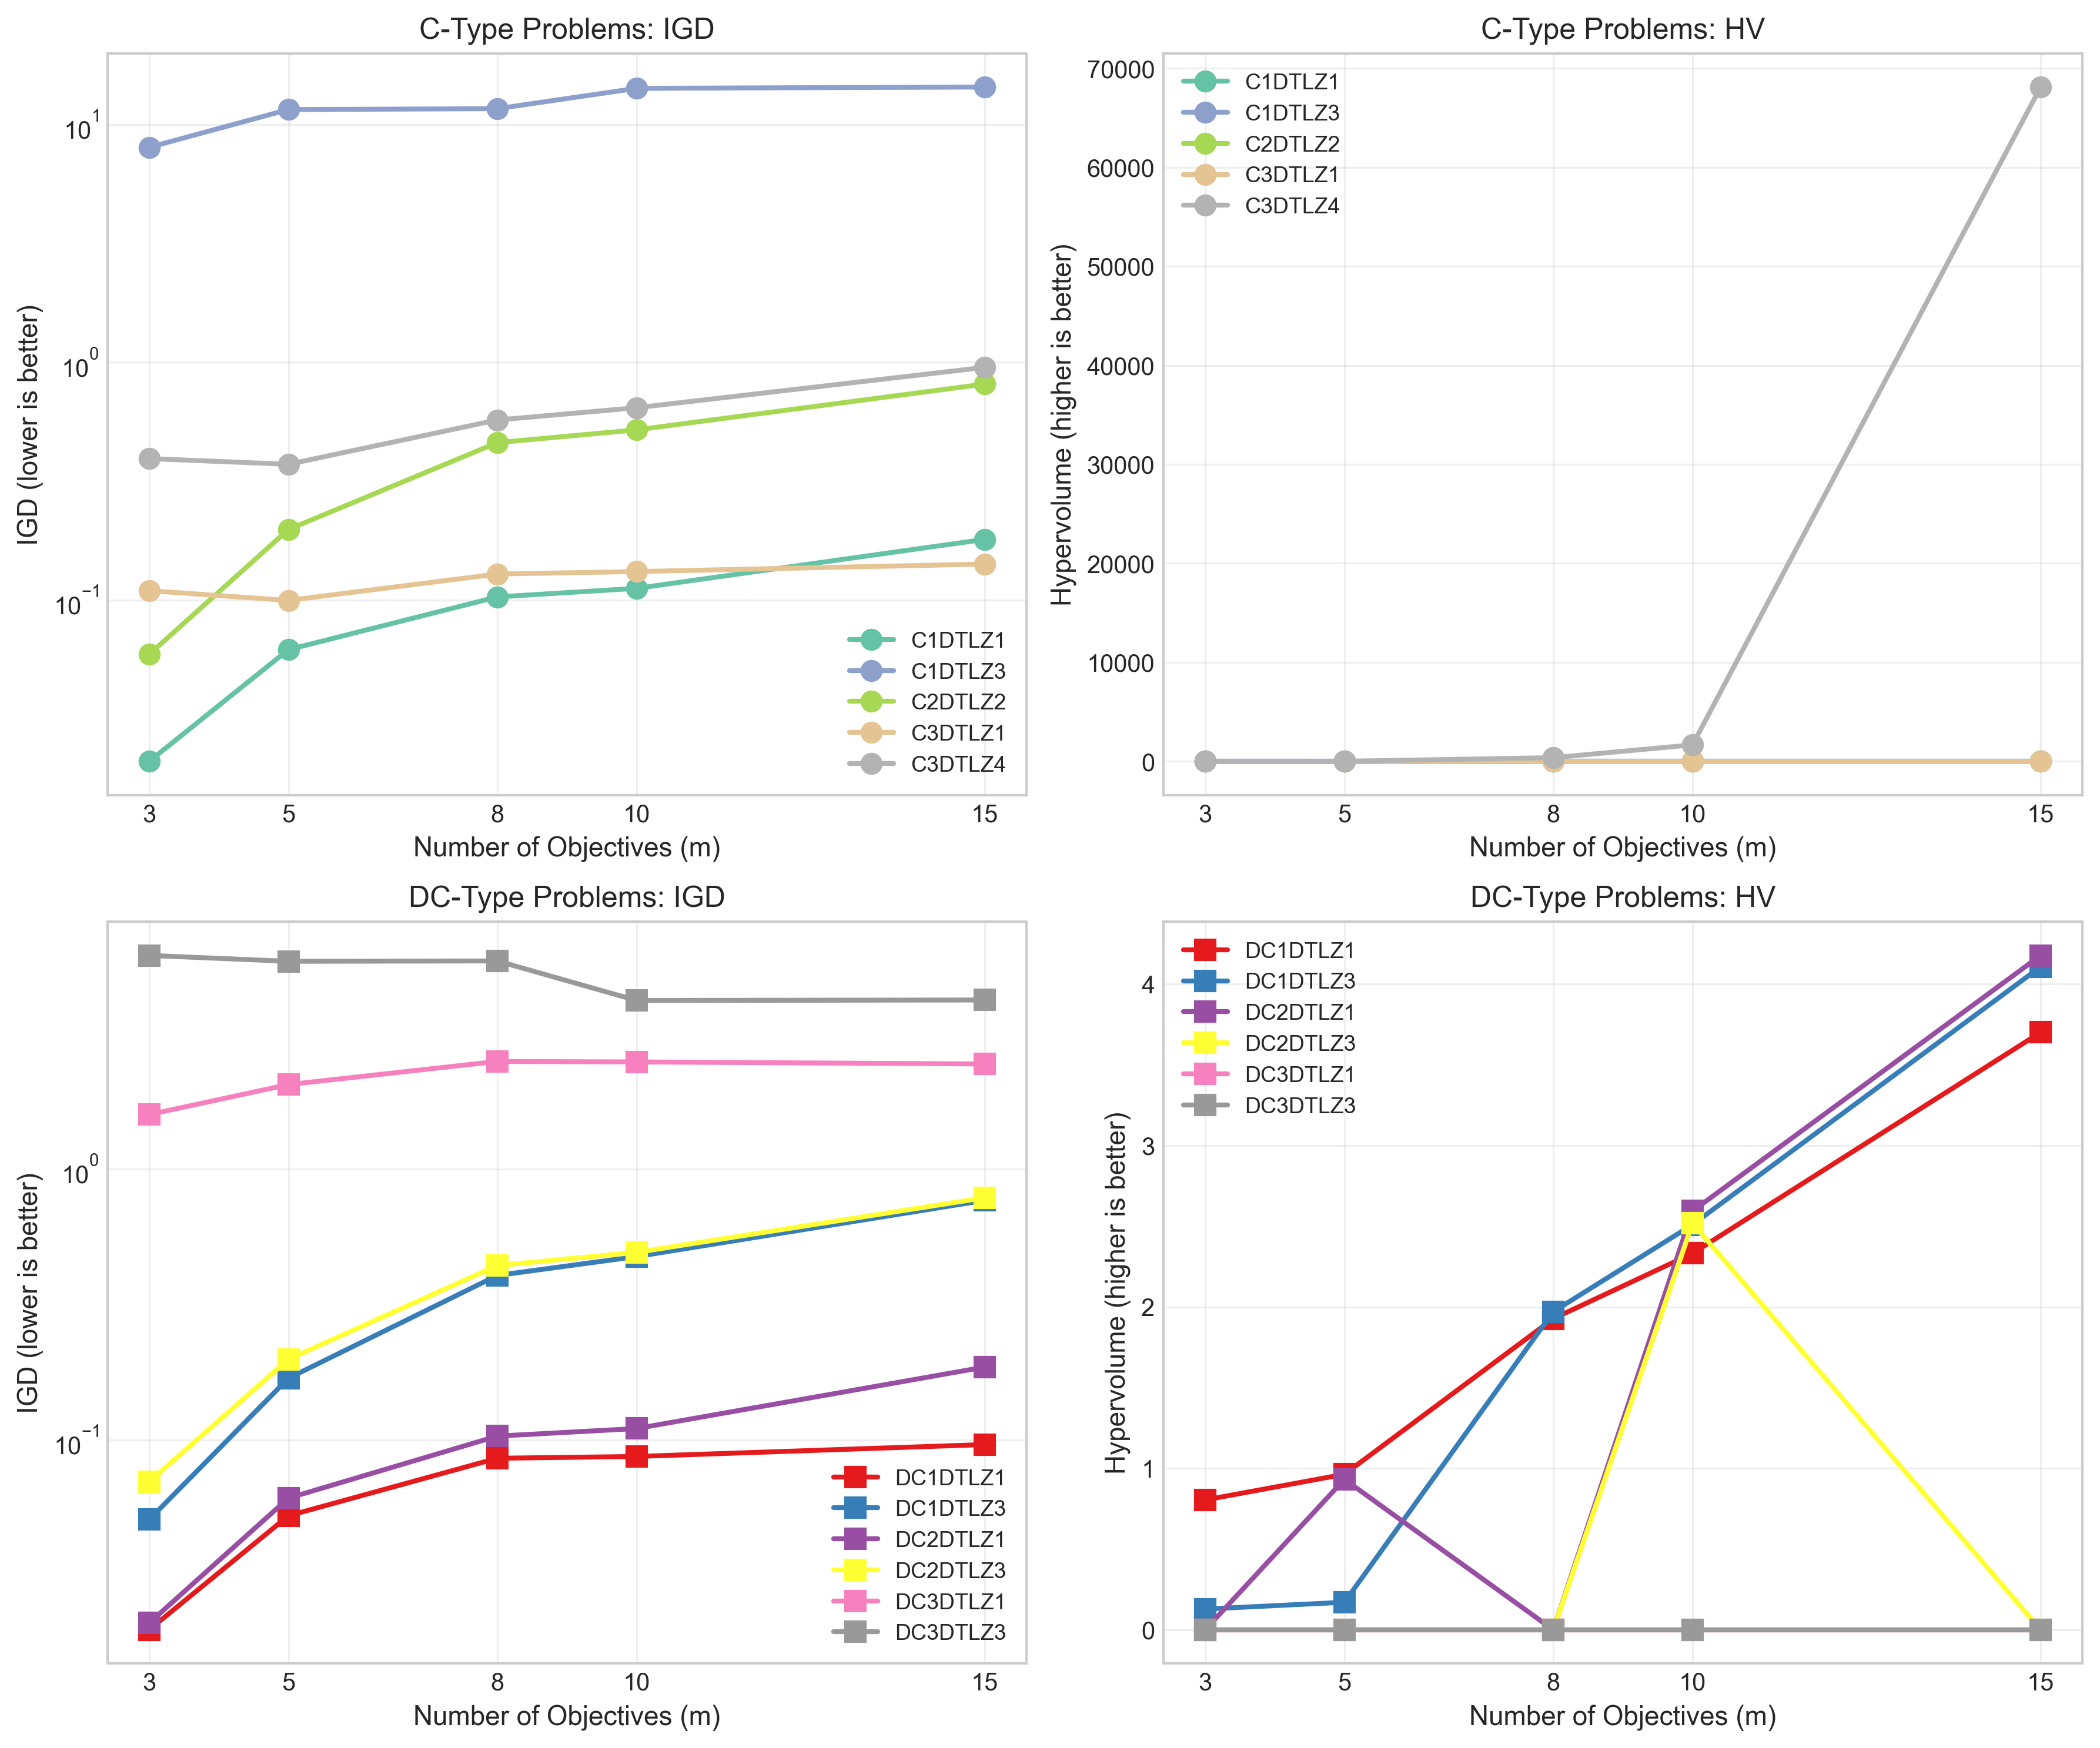
\includegraphics[width=0.85\textwidth]{c_vs_dc_problems.png}
    \caption{IGD for C vs DC problems}
\end{figure}

\begin{figure}[h!]
    \centering
    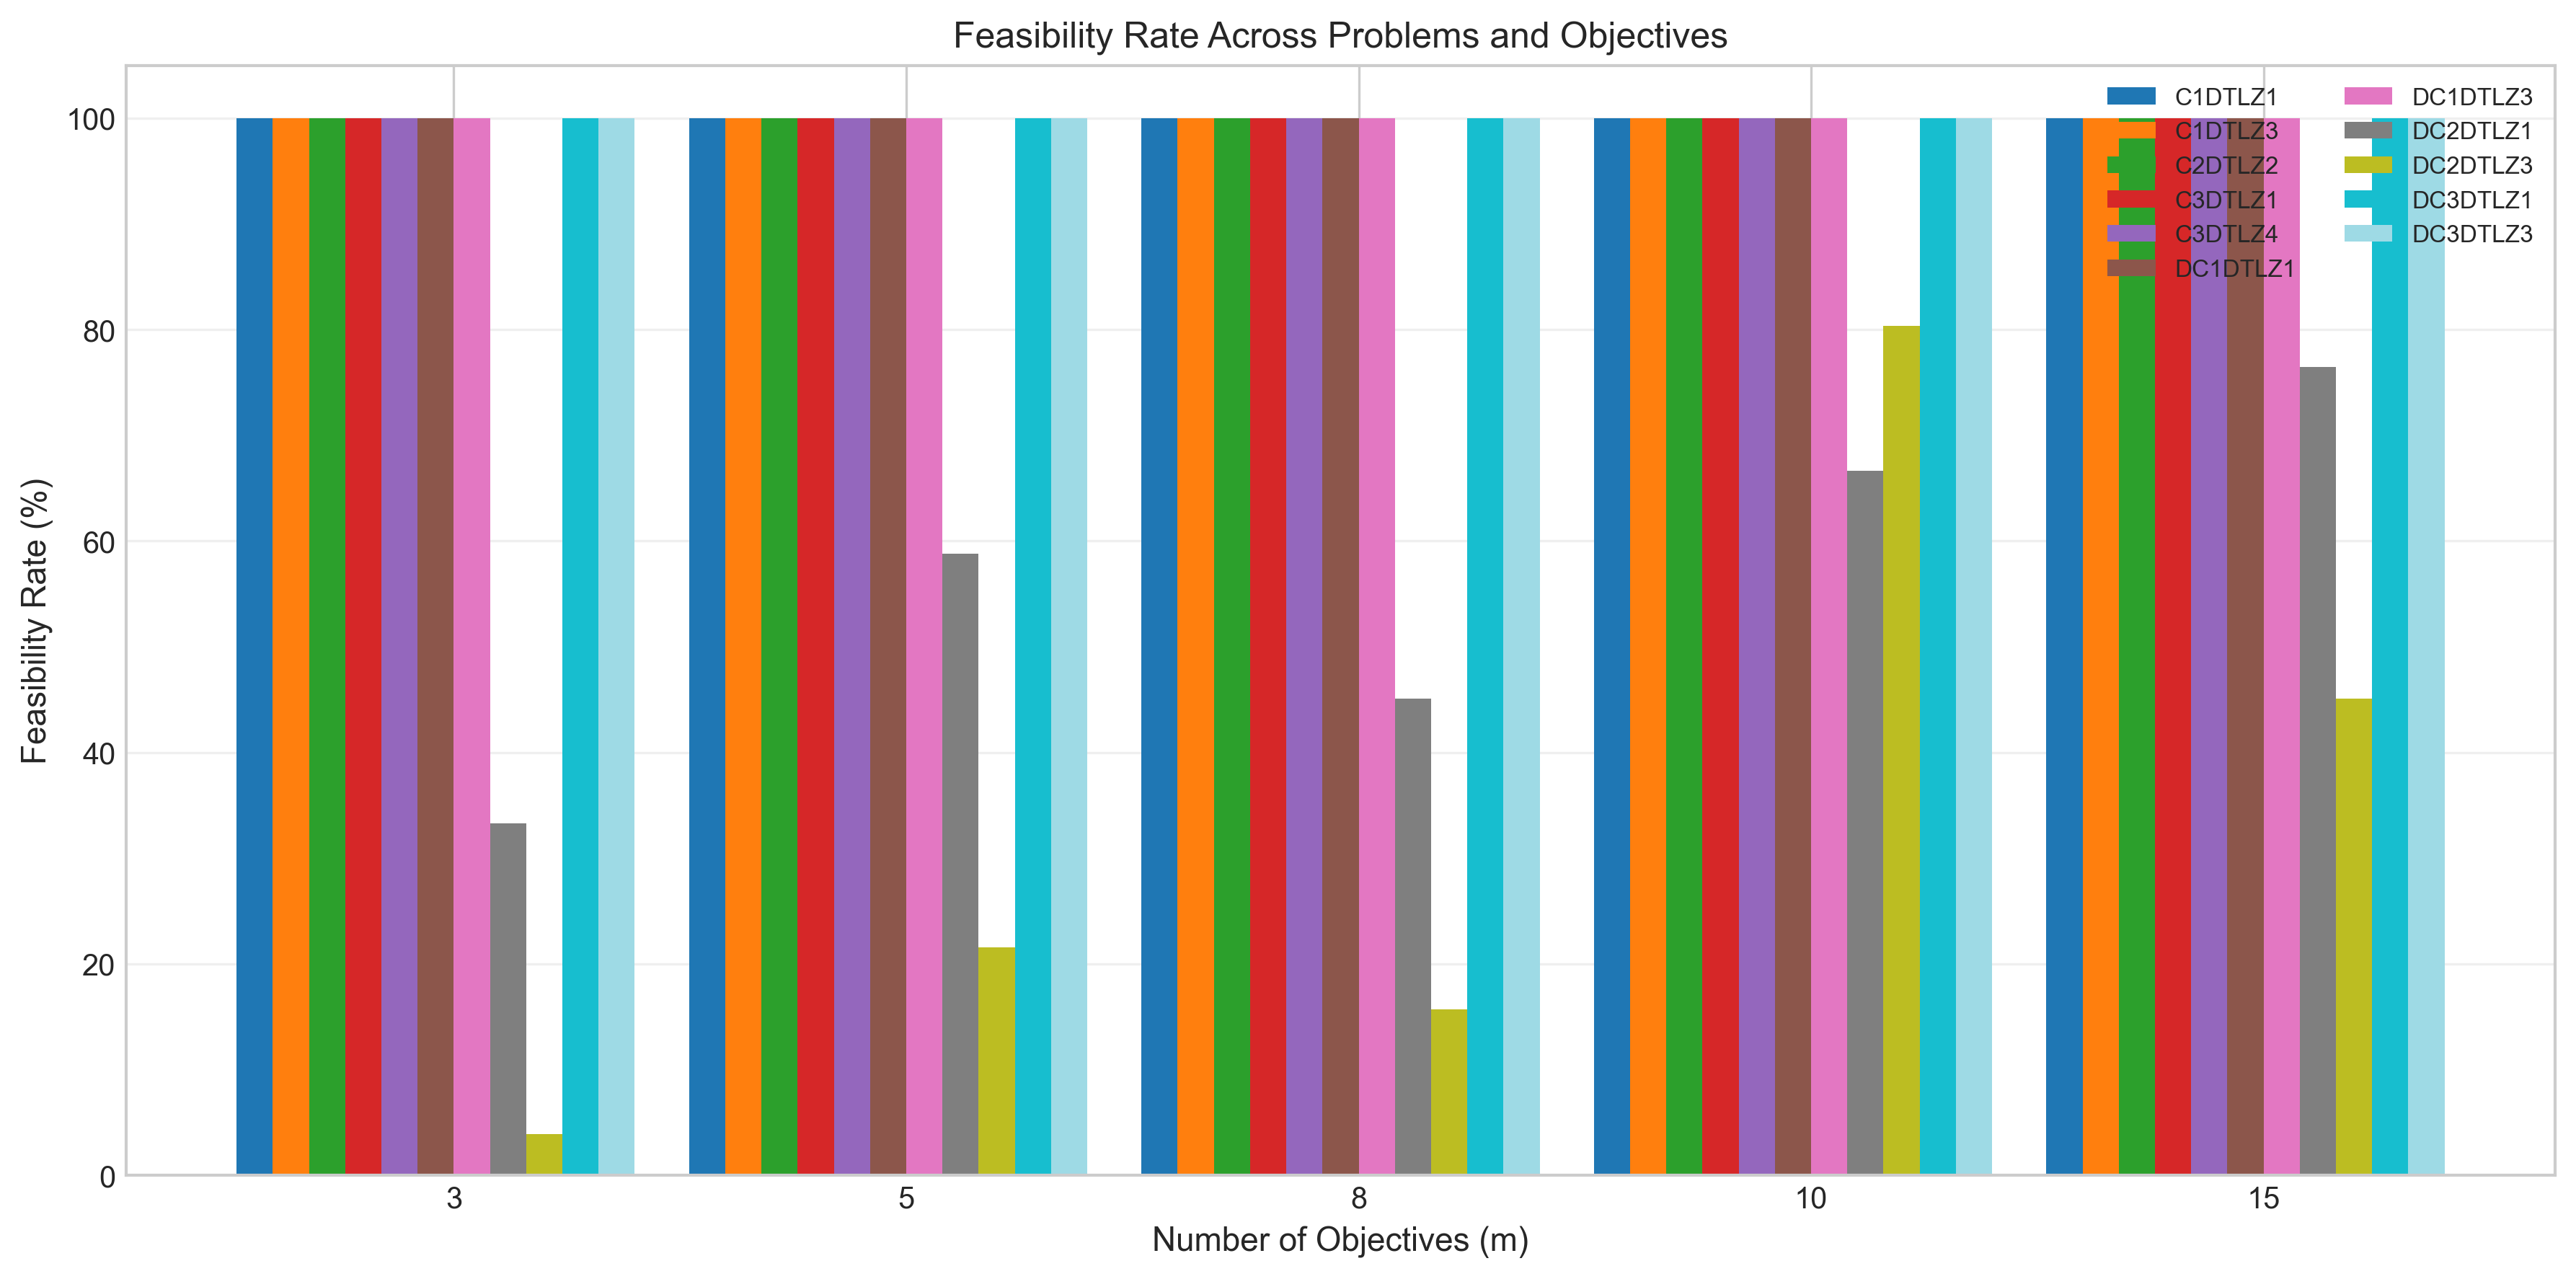
\includegraphics[width=0.85\textwidth]{feasibility_rate.png}
    \caption{Feasibility Rates Across Problems and Objectives}
\end{figure}

\begin{figure}[h!]
    \centering
    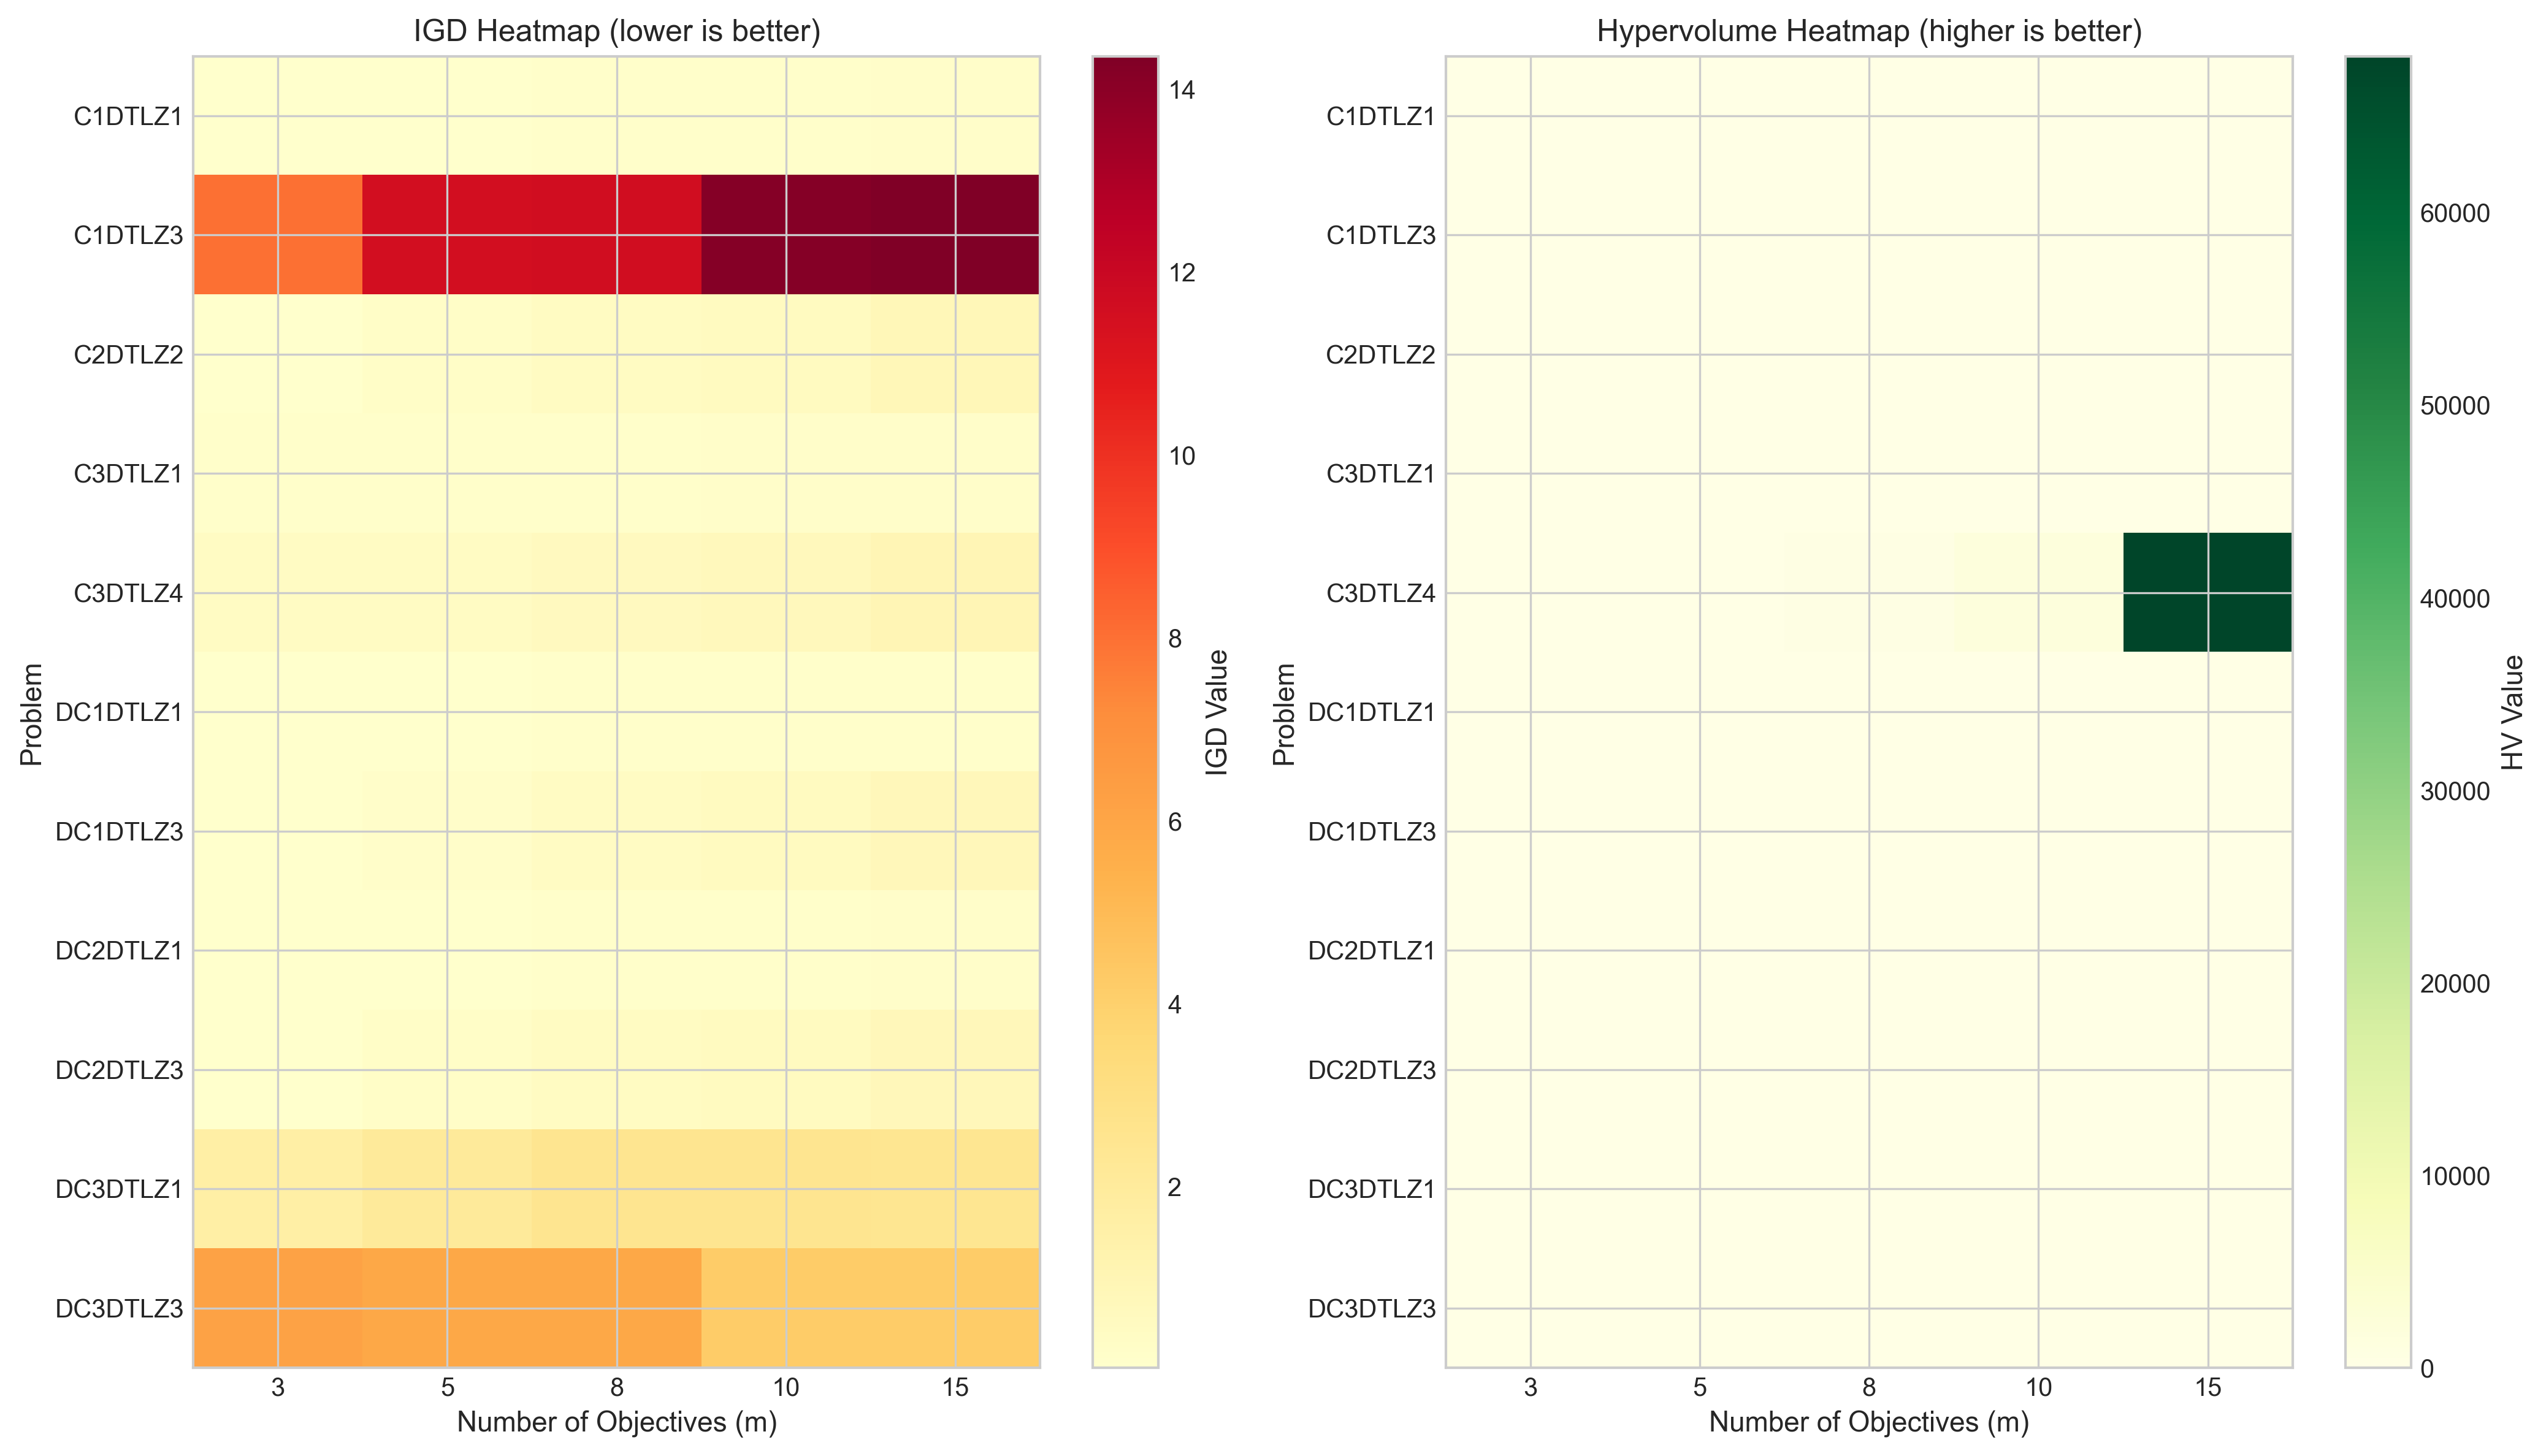
\includegraphics[width=0.85\textwidth]{heatmap_metrics.png}
    \caption{IGD and HV Heatmaps across problems}
\end{figure}

\begin{figure}[h!]
    \centering
    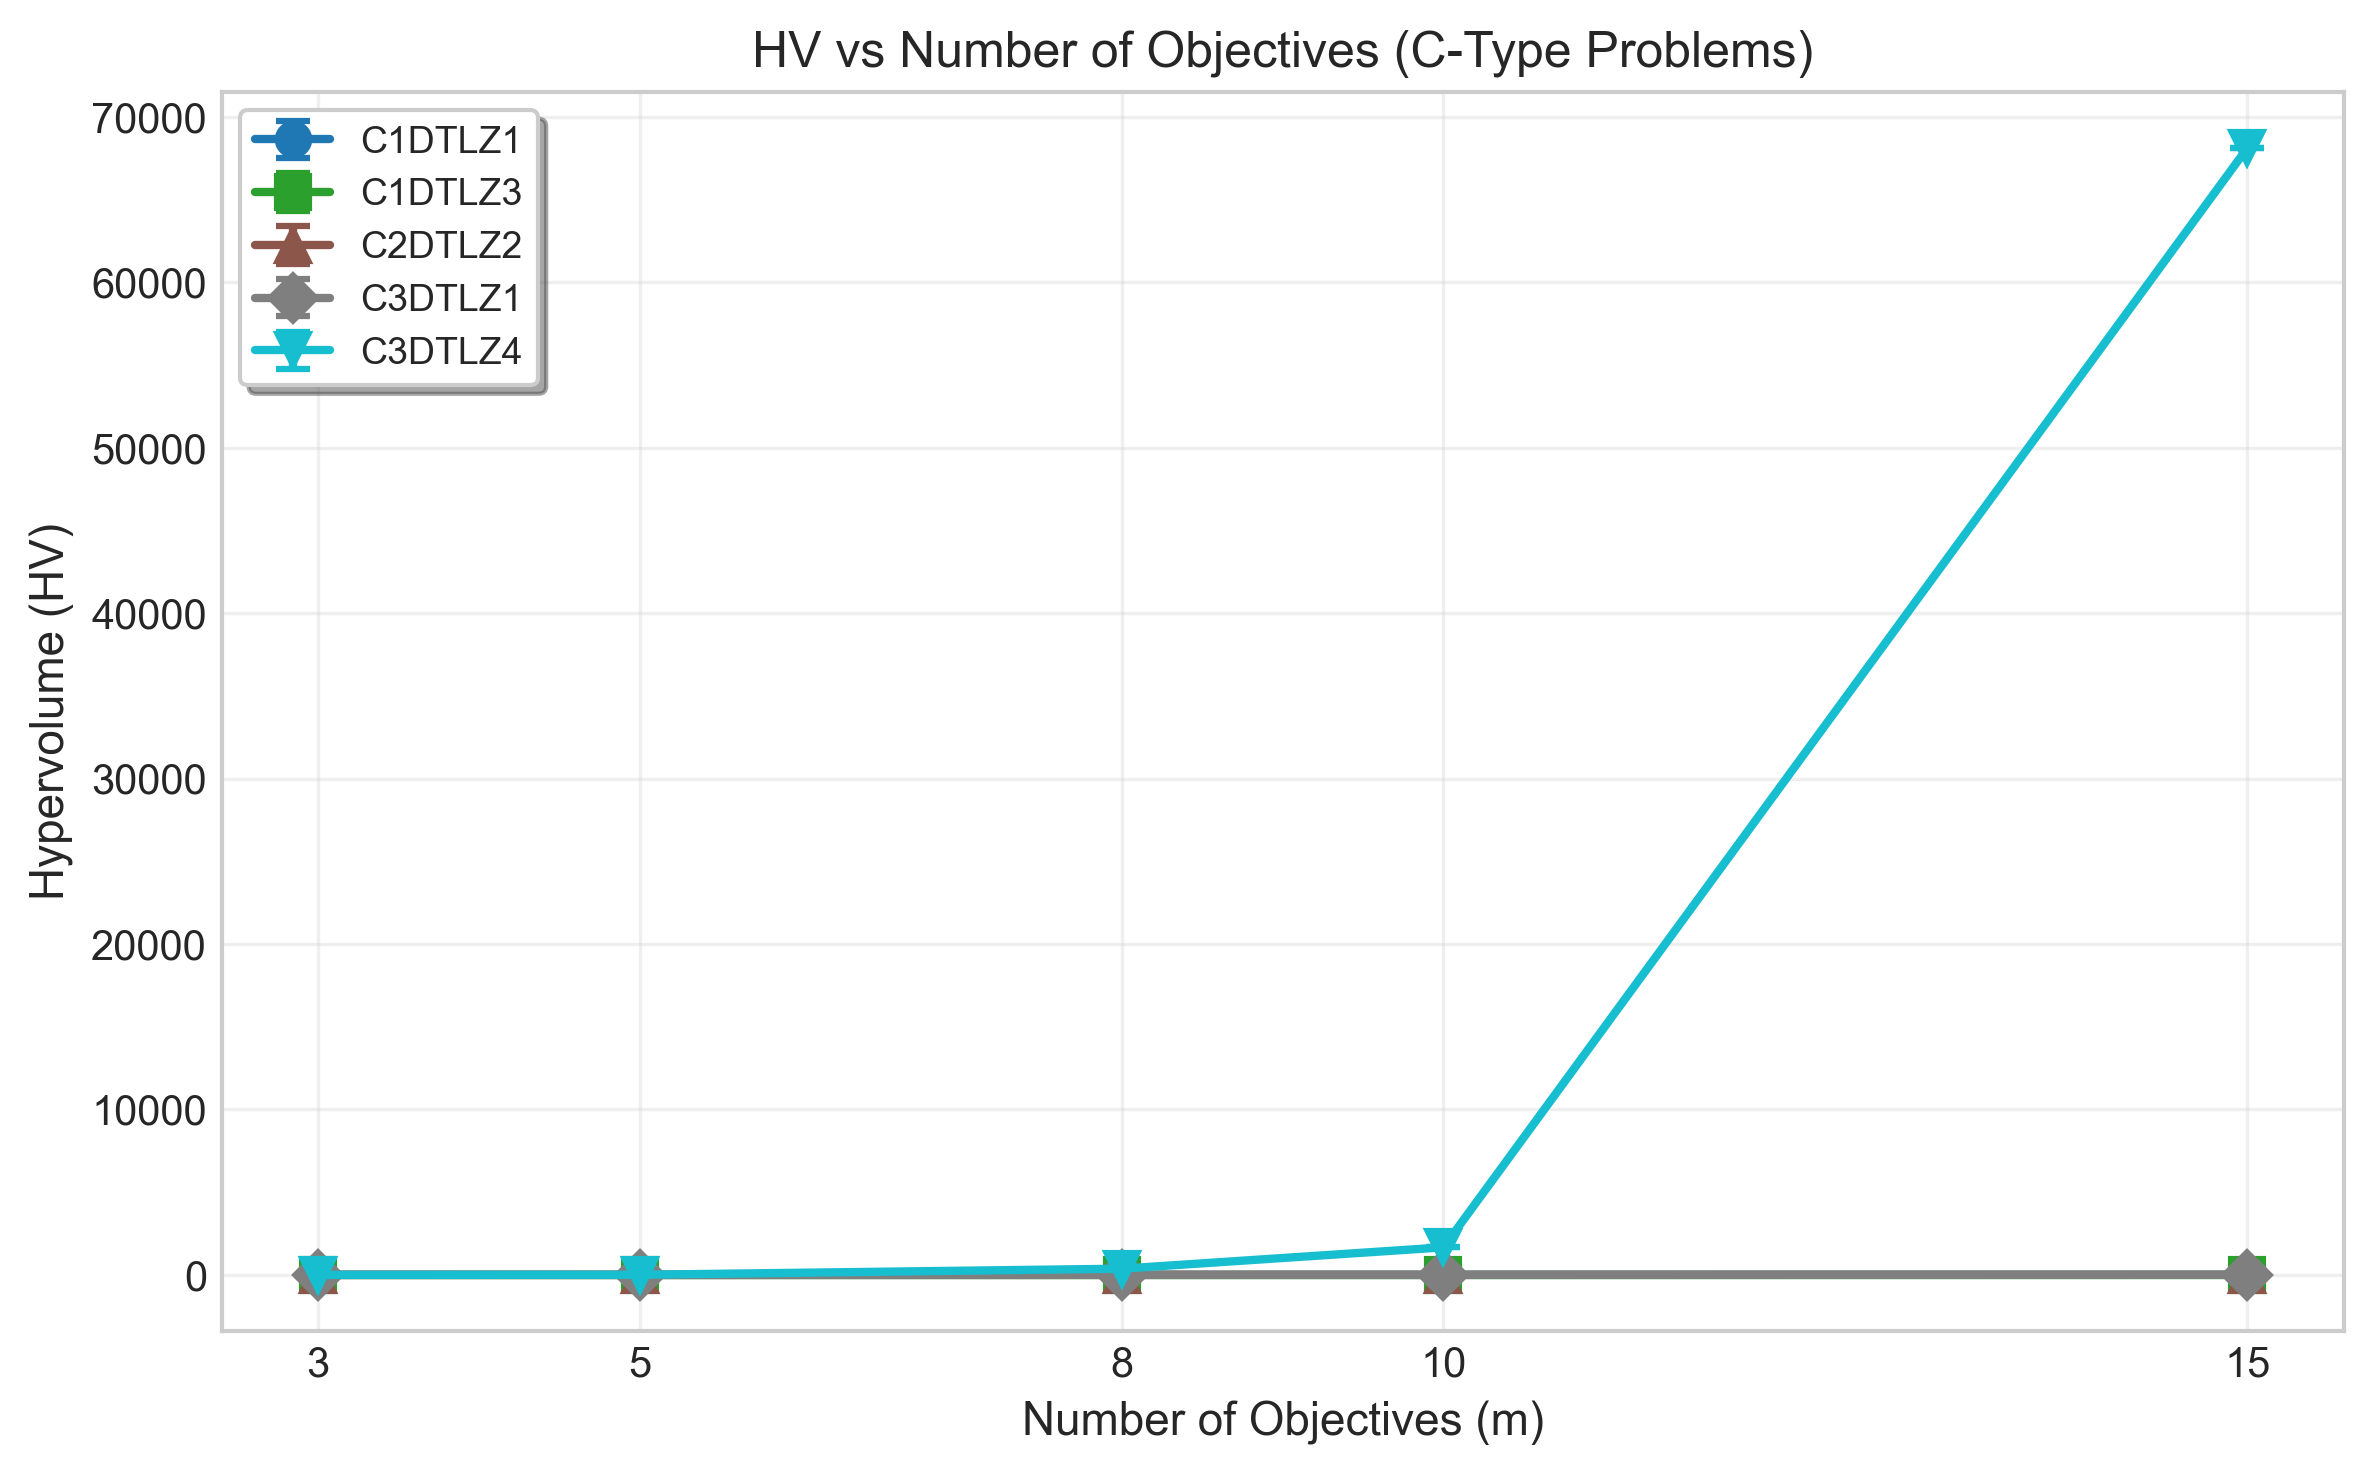
\includegraphics[width=0.85\textwidth]{hv_vs_objectives_c_type.png}
    \caption{HV vs Number of Objectives (C-type)}
\end{figure}

\begin{figure}[h!]
    \centering
    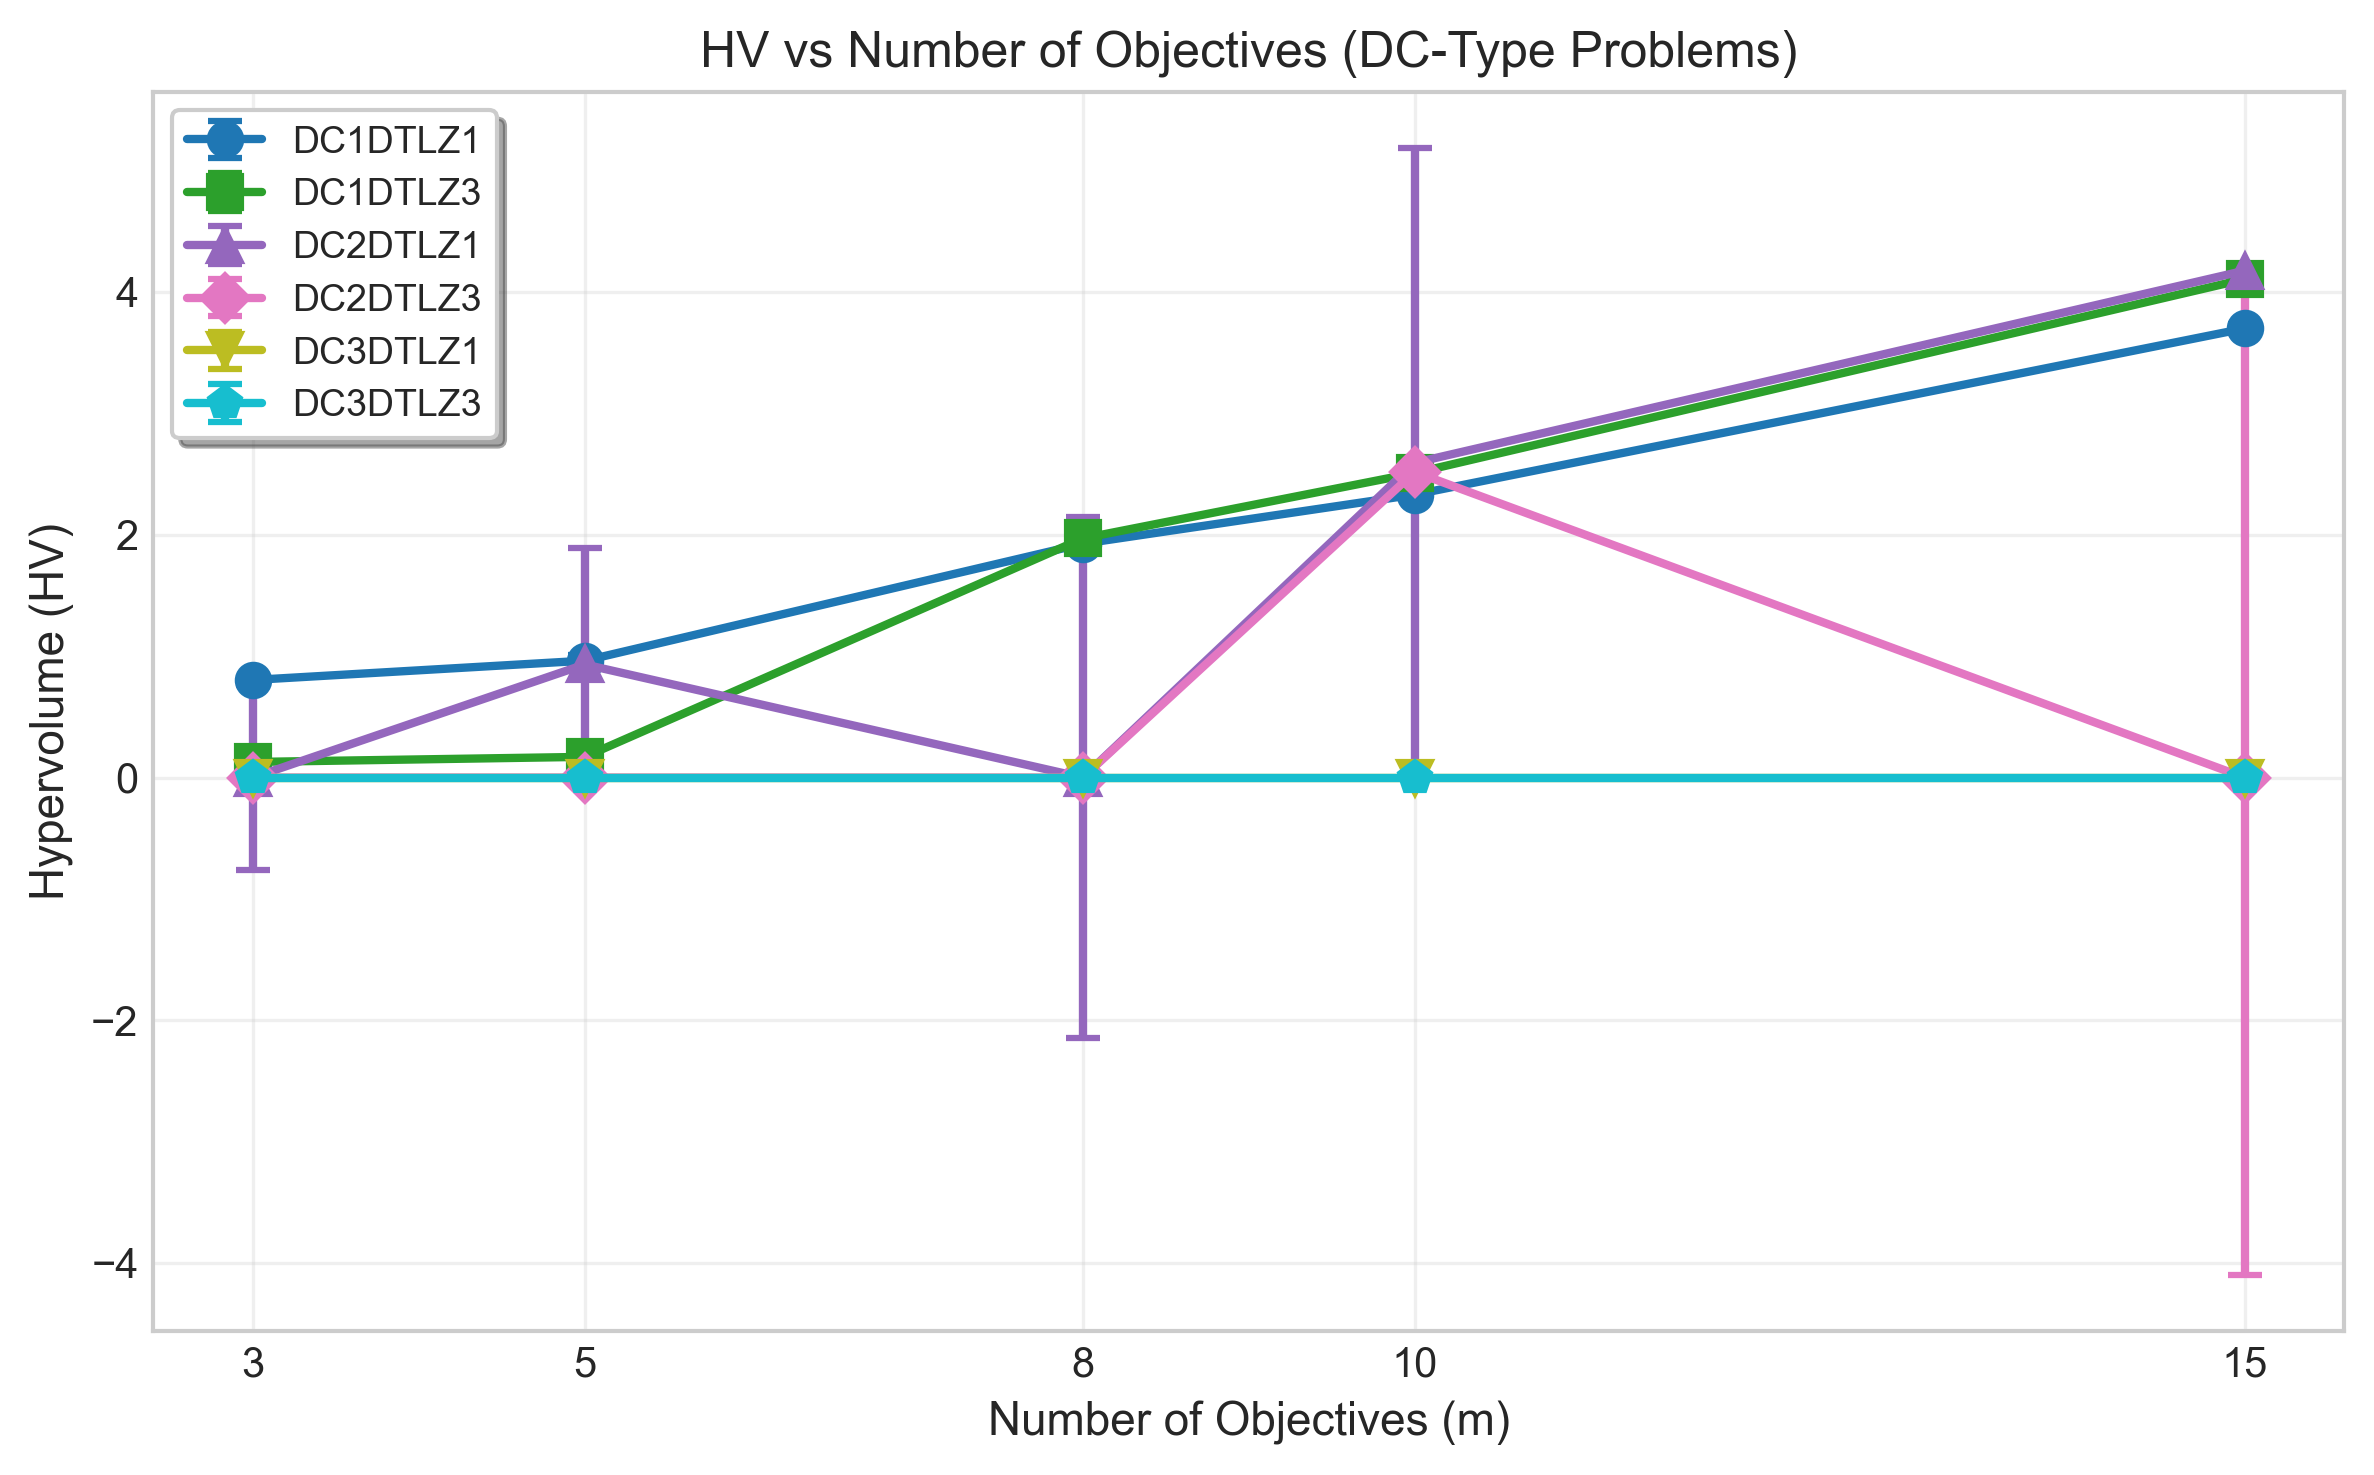
\includegraphics[width=0.85\textwidth]{hv_vs_objectives_dc_type.png}
    \caption{HV vs Number of Objectives (DC-type)}
\end{figure}

\begin{figure}[h!]
    \centering
    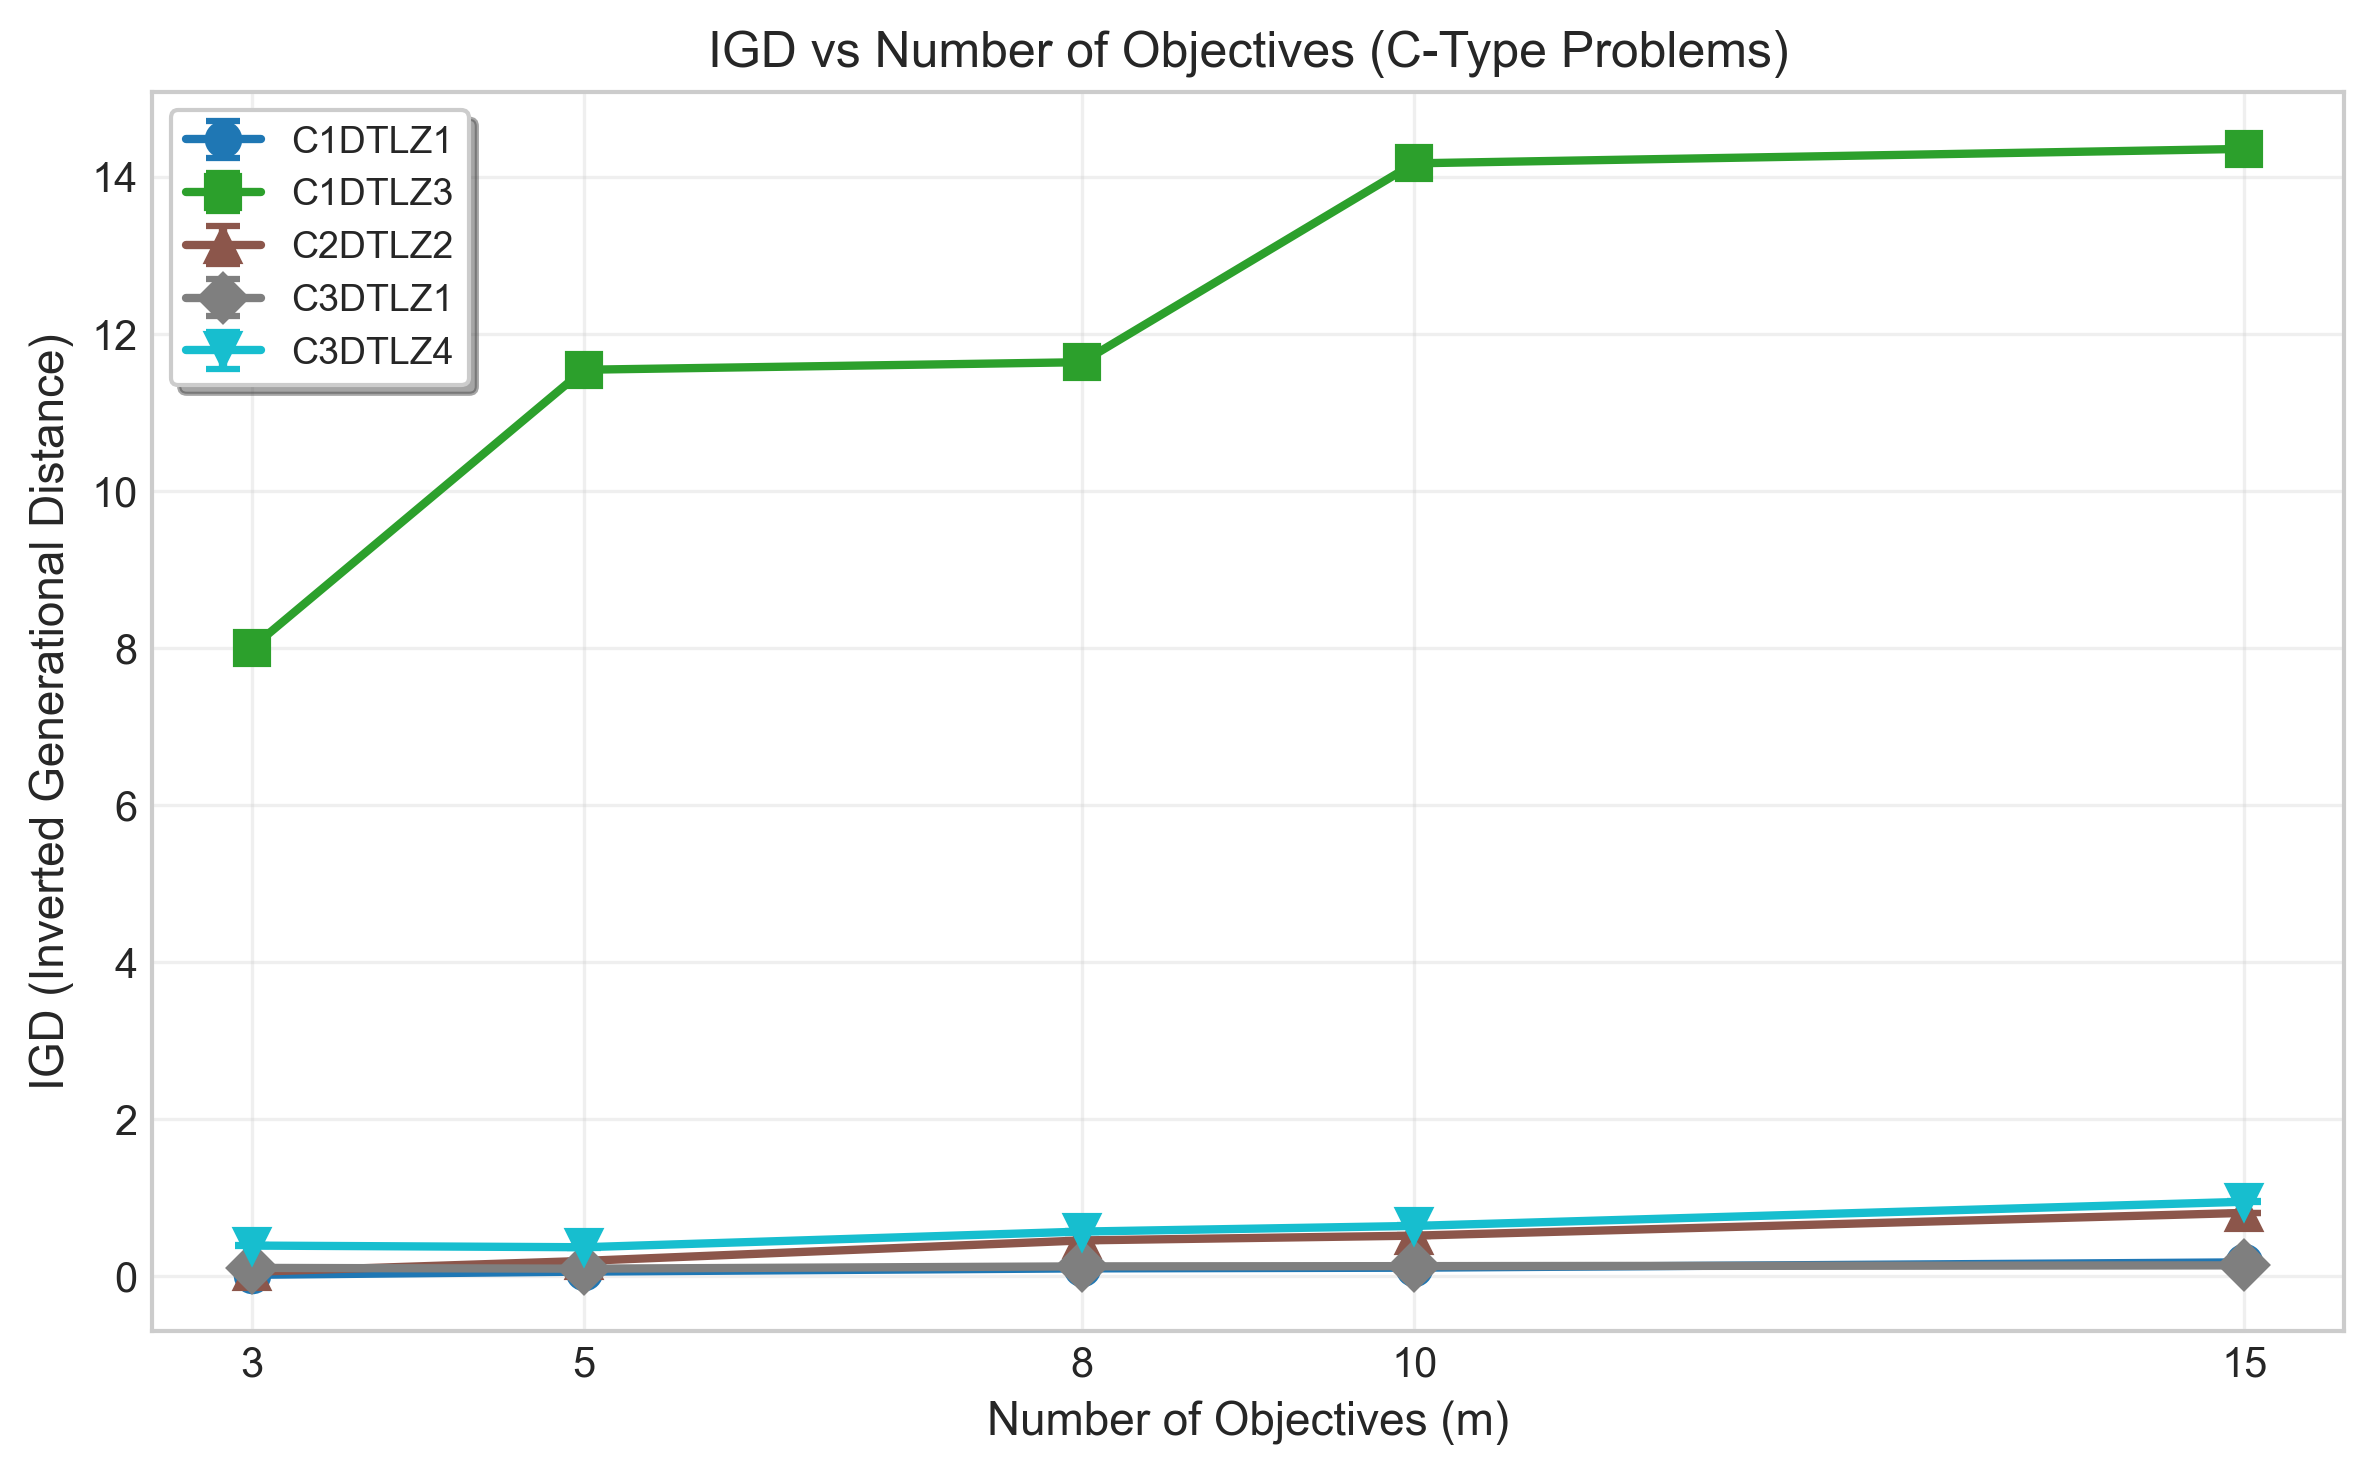
\includegraphics[width=0.85\textwidth]{igd_vs_objectives_c_type.png}
    \caption{IGD vs Number of Objectives (C-type)}
\end{figure}

\begin{figure}[h!]
    \centering
    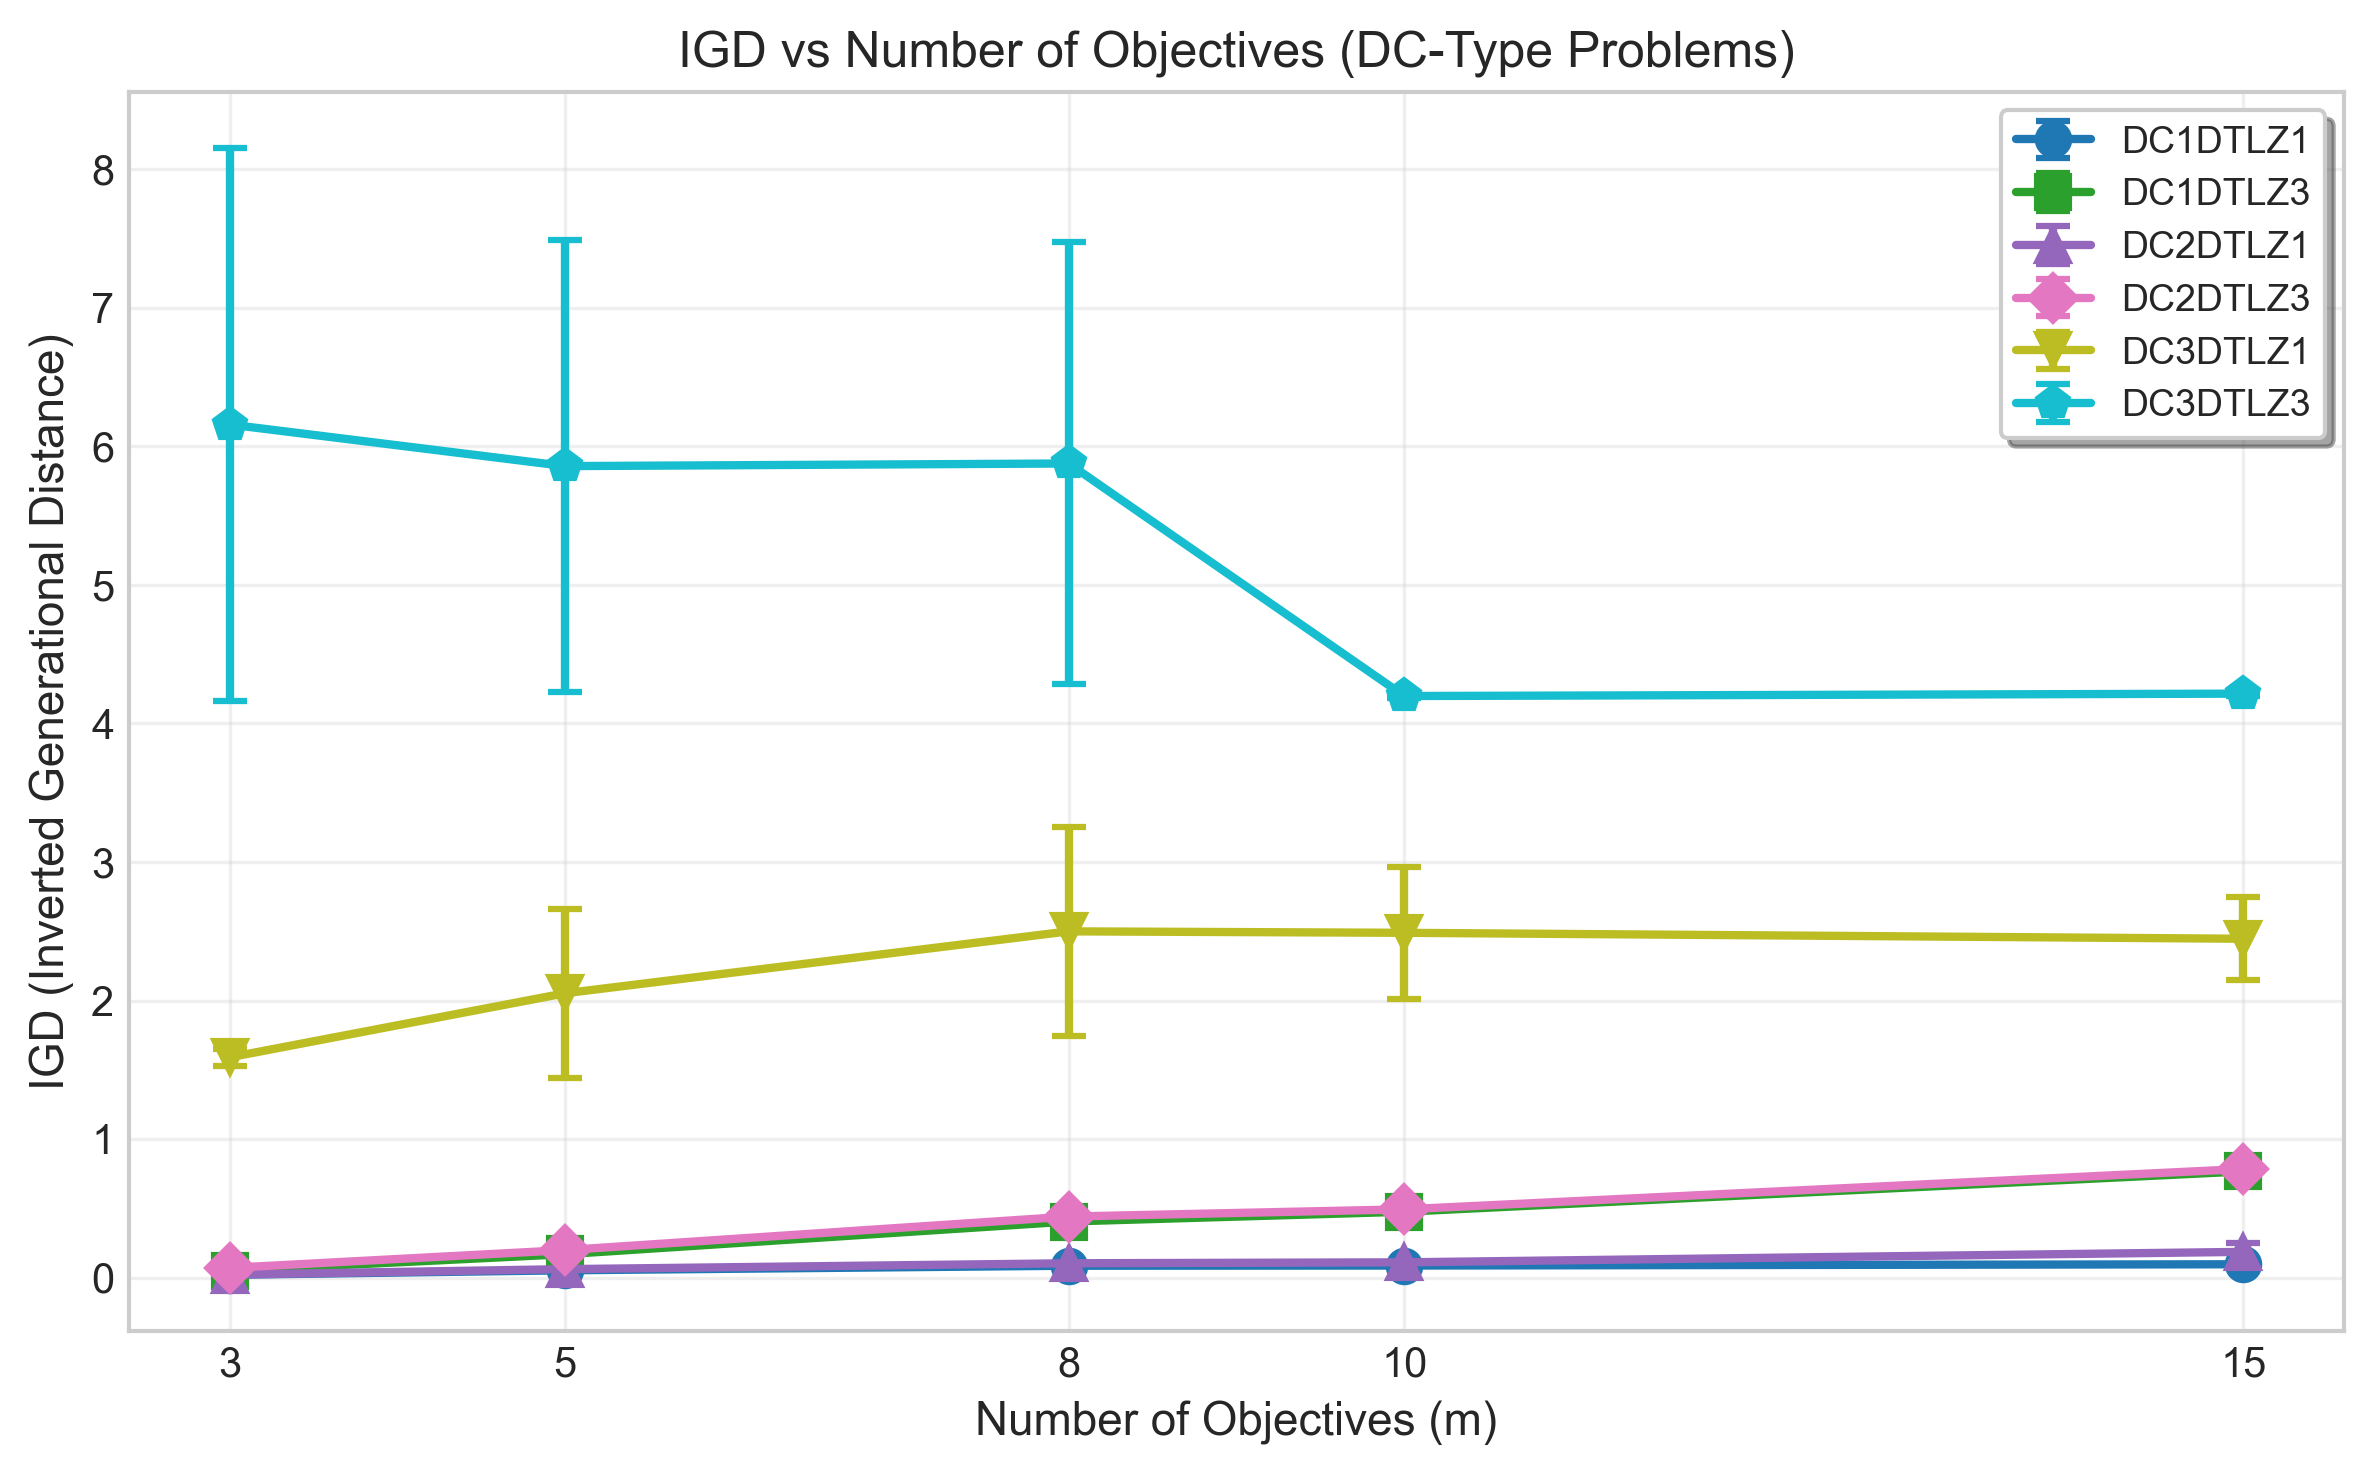
\includegraphics[width=0.85\textwidth]{igd_vs_objectives_dc_type.png}
    \caption{IGD vs Number of Objectives (DC-type)}
\end{figure}

\begin{figure}[h!]
    \centering
    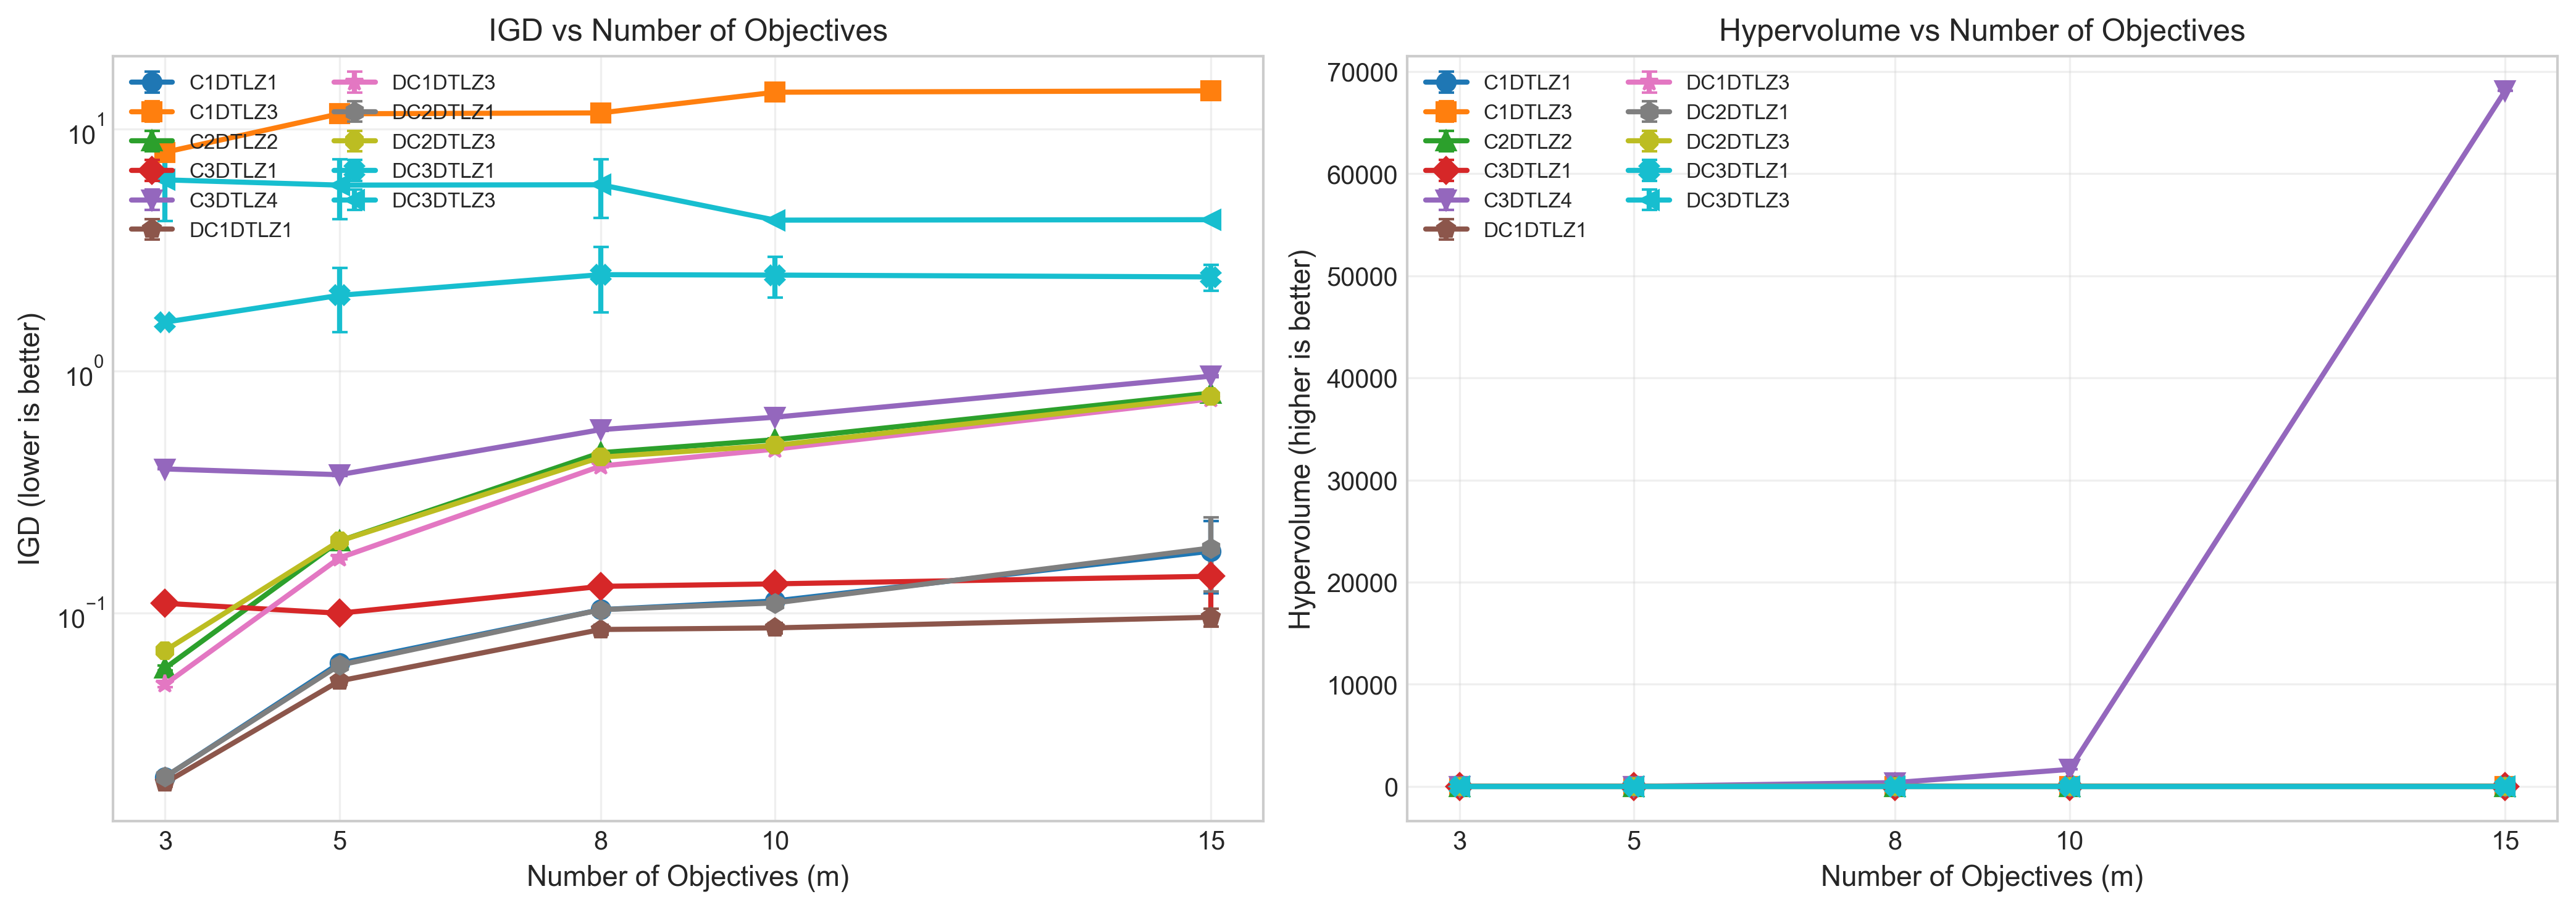
\includegraphics[width=0.85\textwidth]{igd_hv_comparison.png}
    \caption{IGD and HV vs Number of Objectives}
\end{figure}


\begin{figure}[h!]
    \centering
    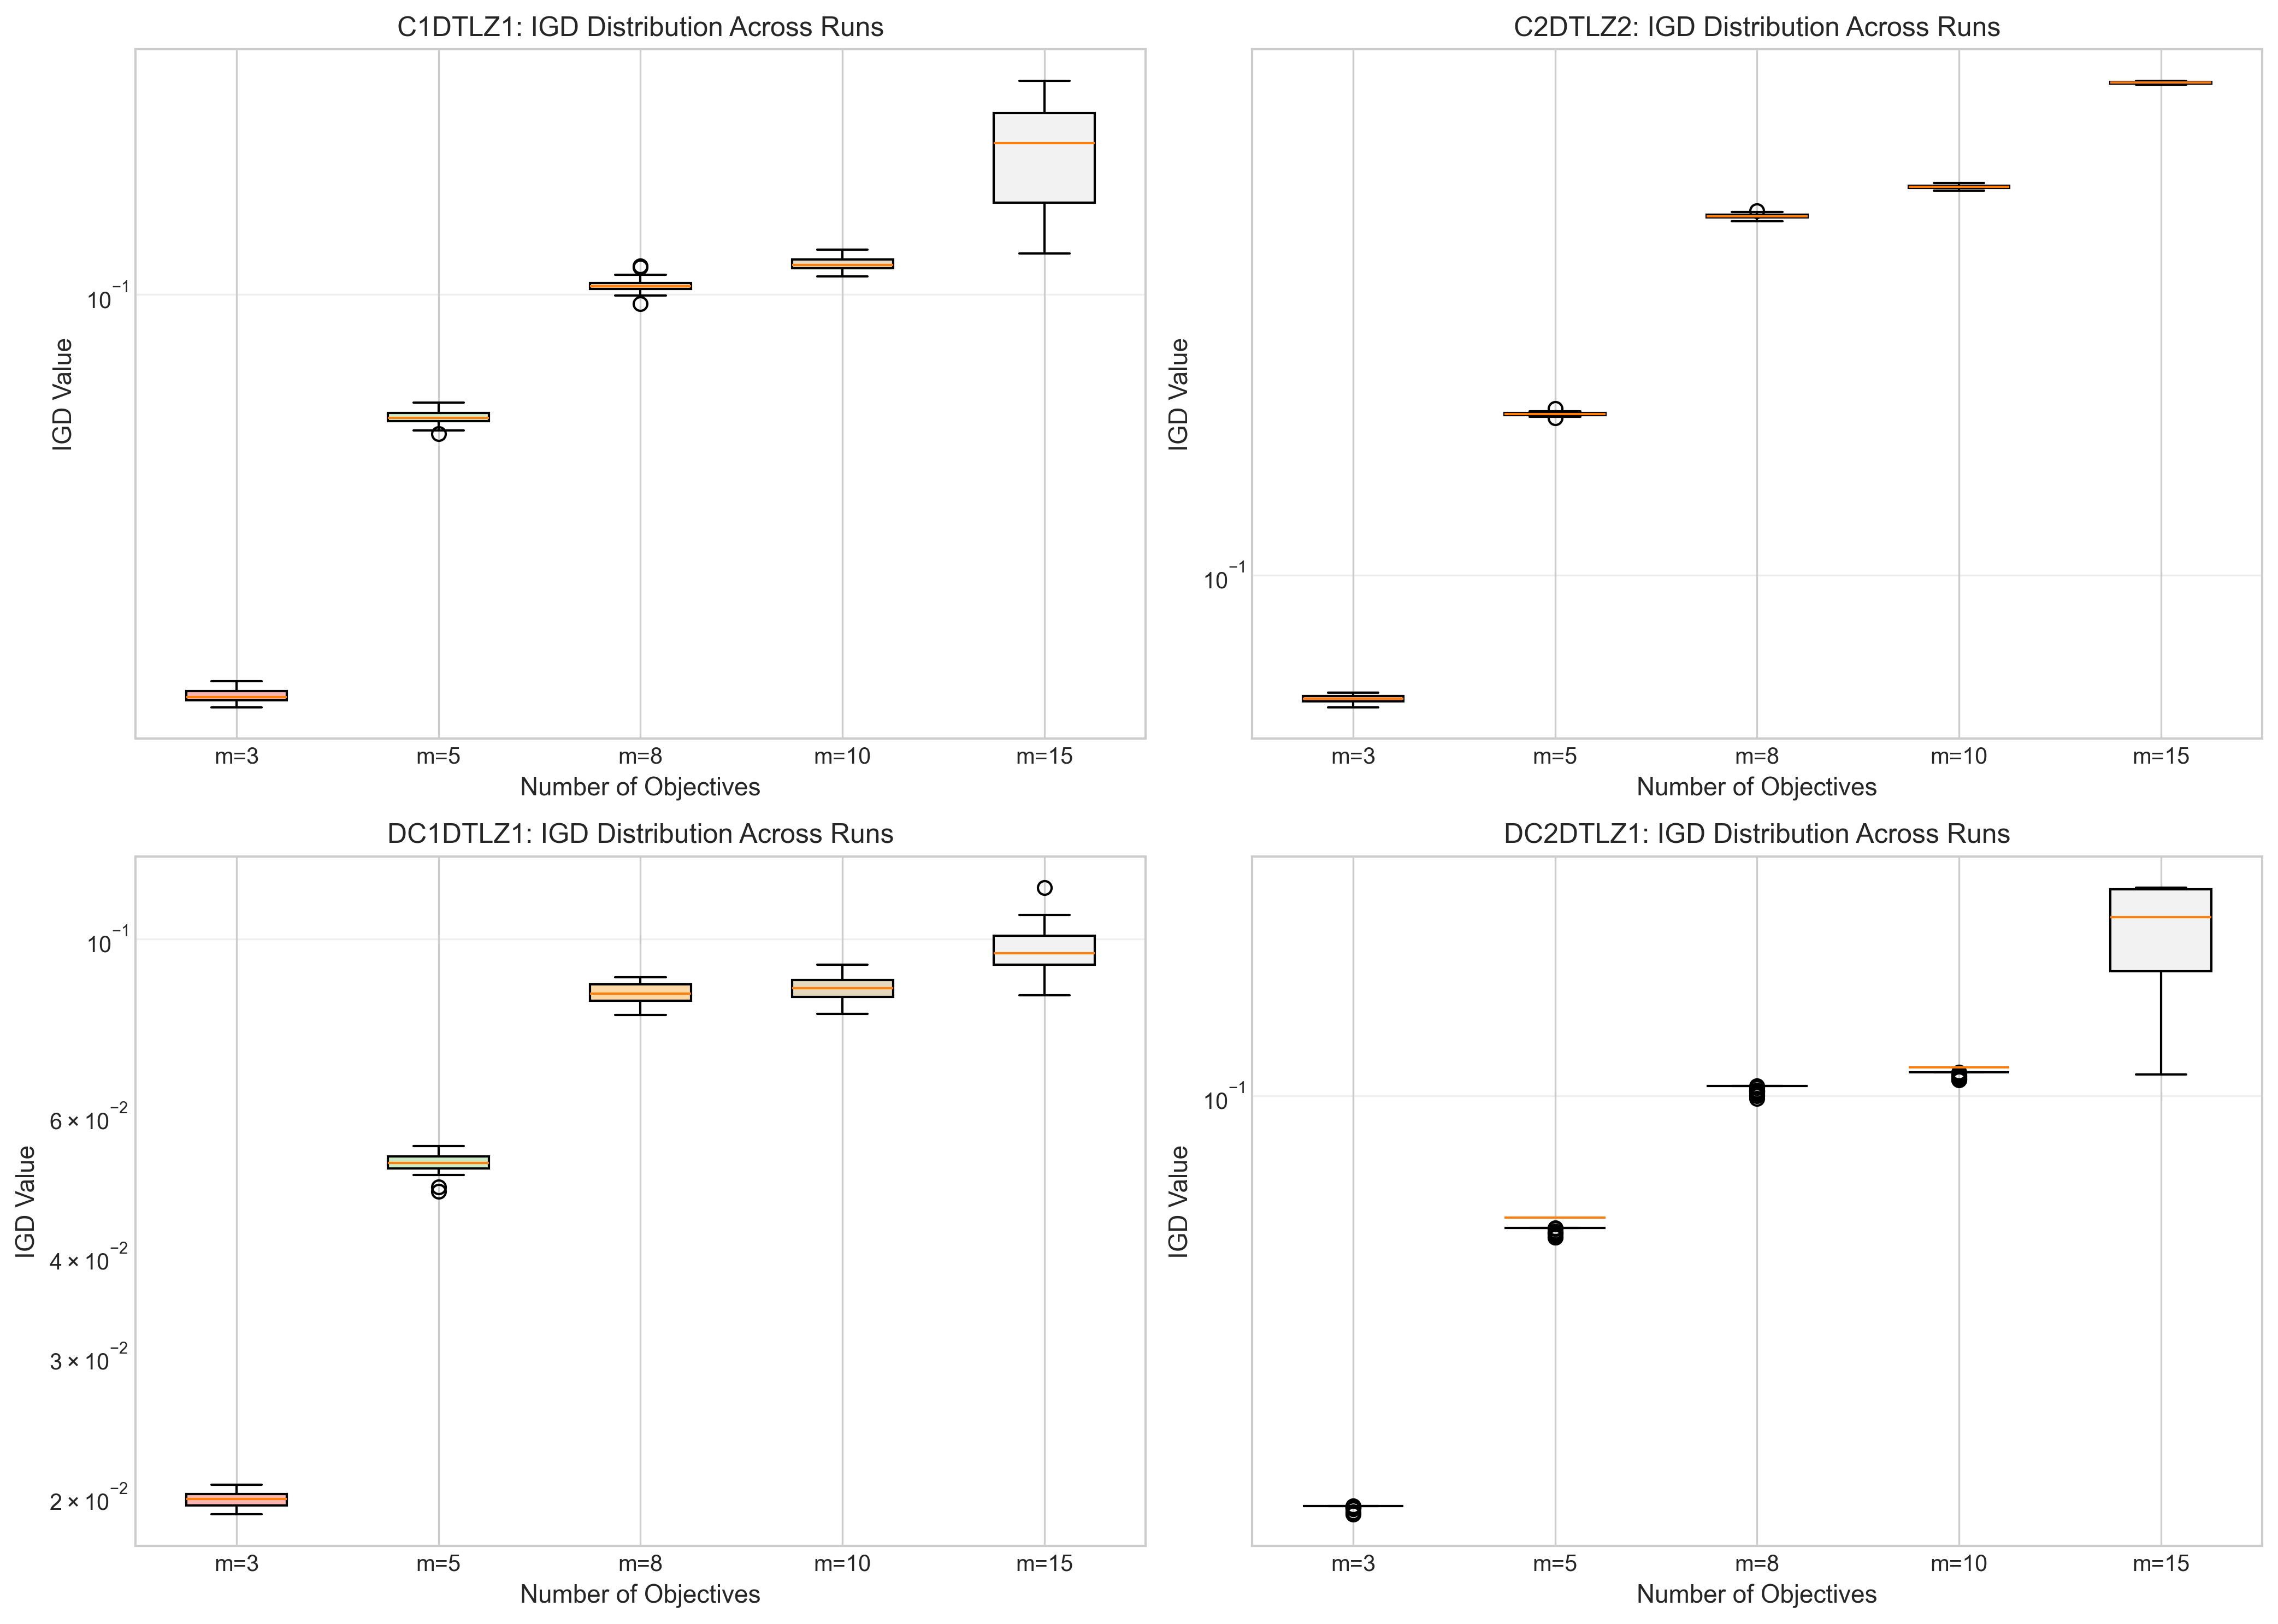
\includegraphics[width=0.85\textwidth]{runs_distribution_igd.png}
    \caption{IGD Distribution across runs}
\end{figure}

\begin{figure}[h!]
    \centering
    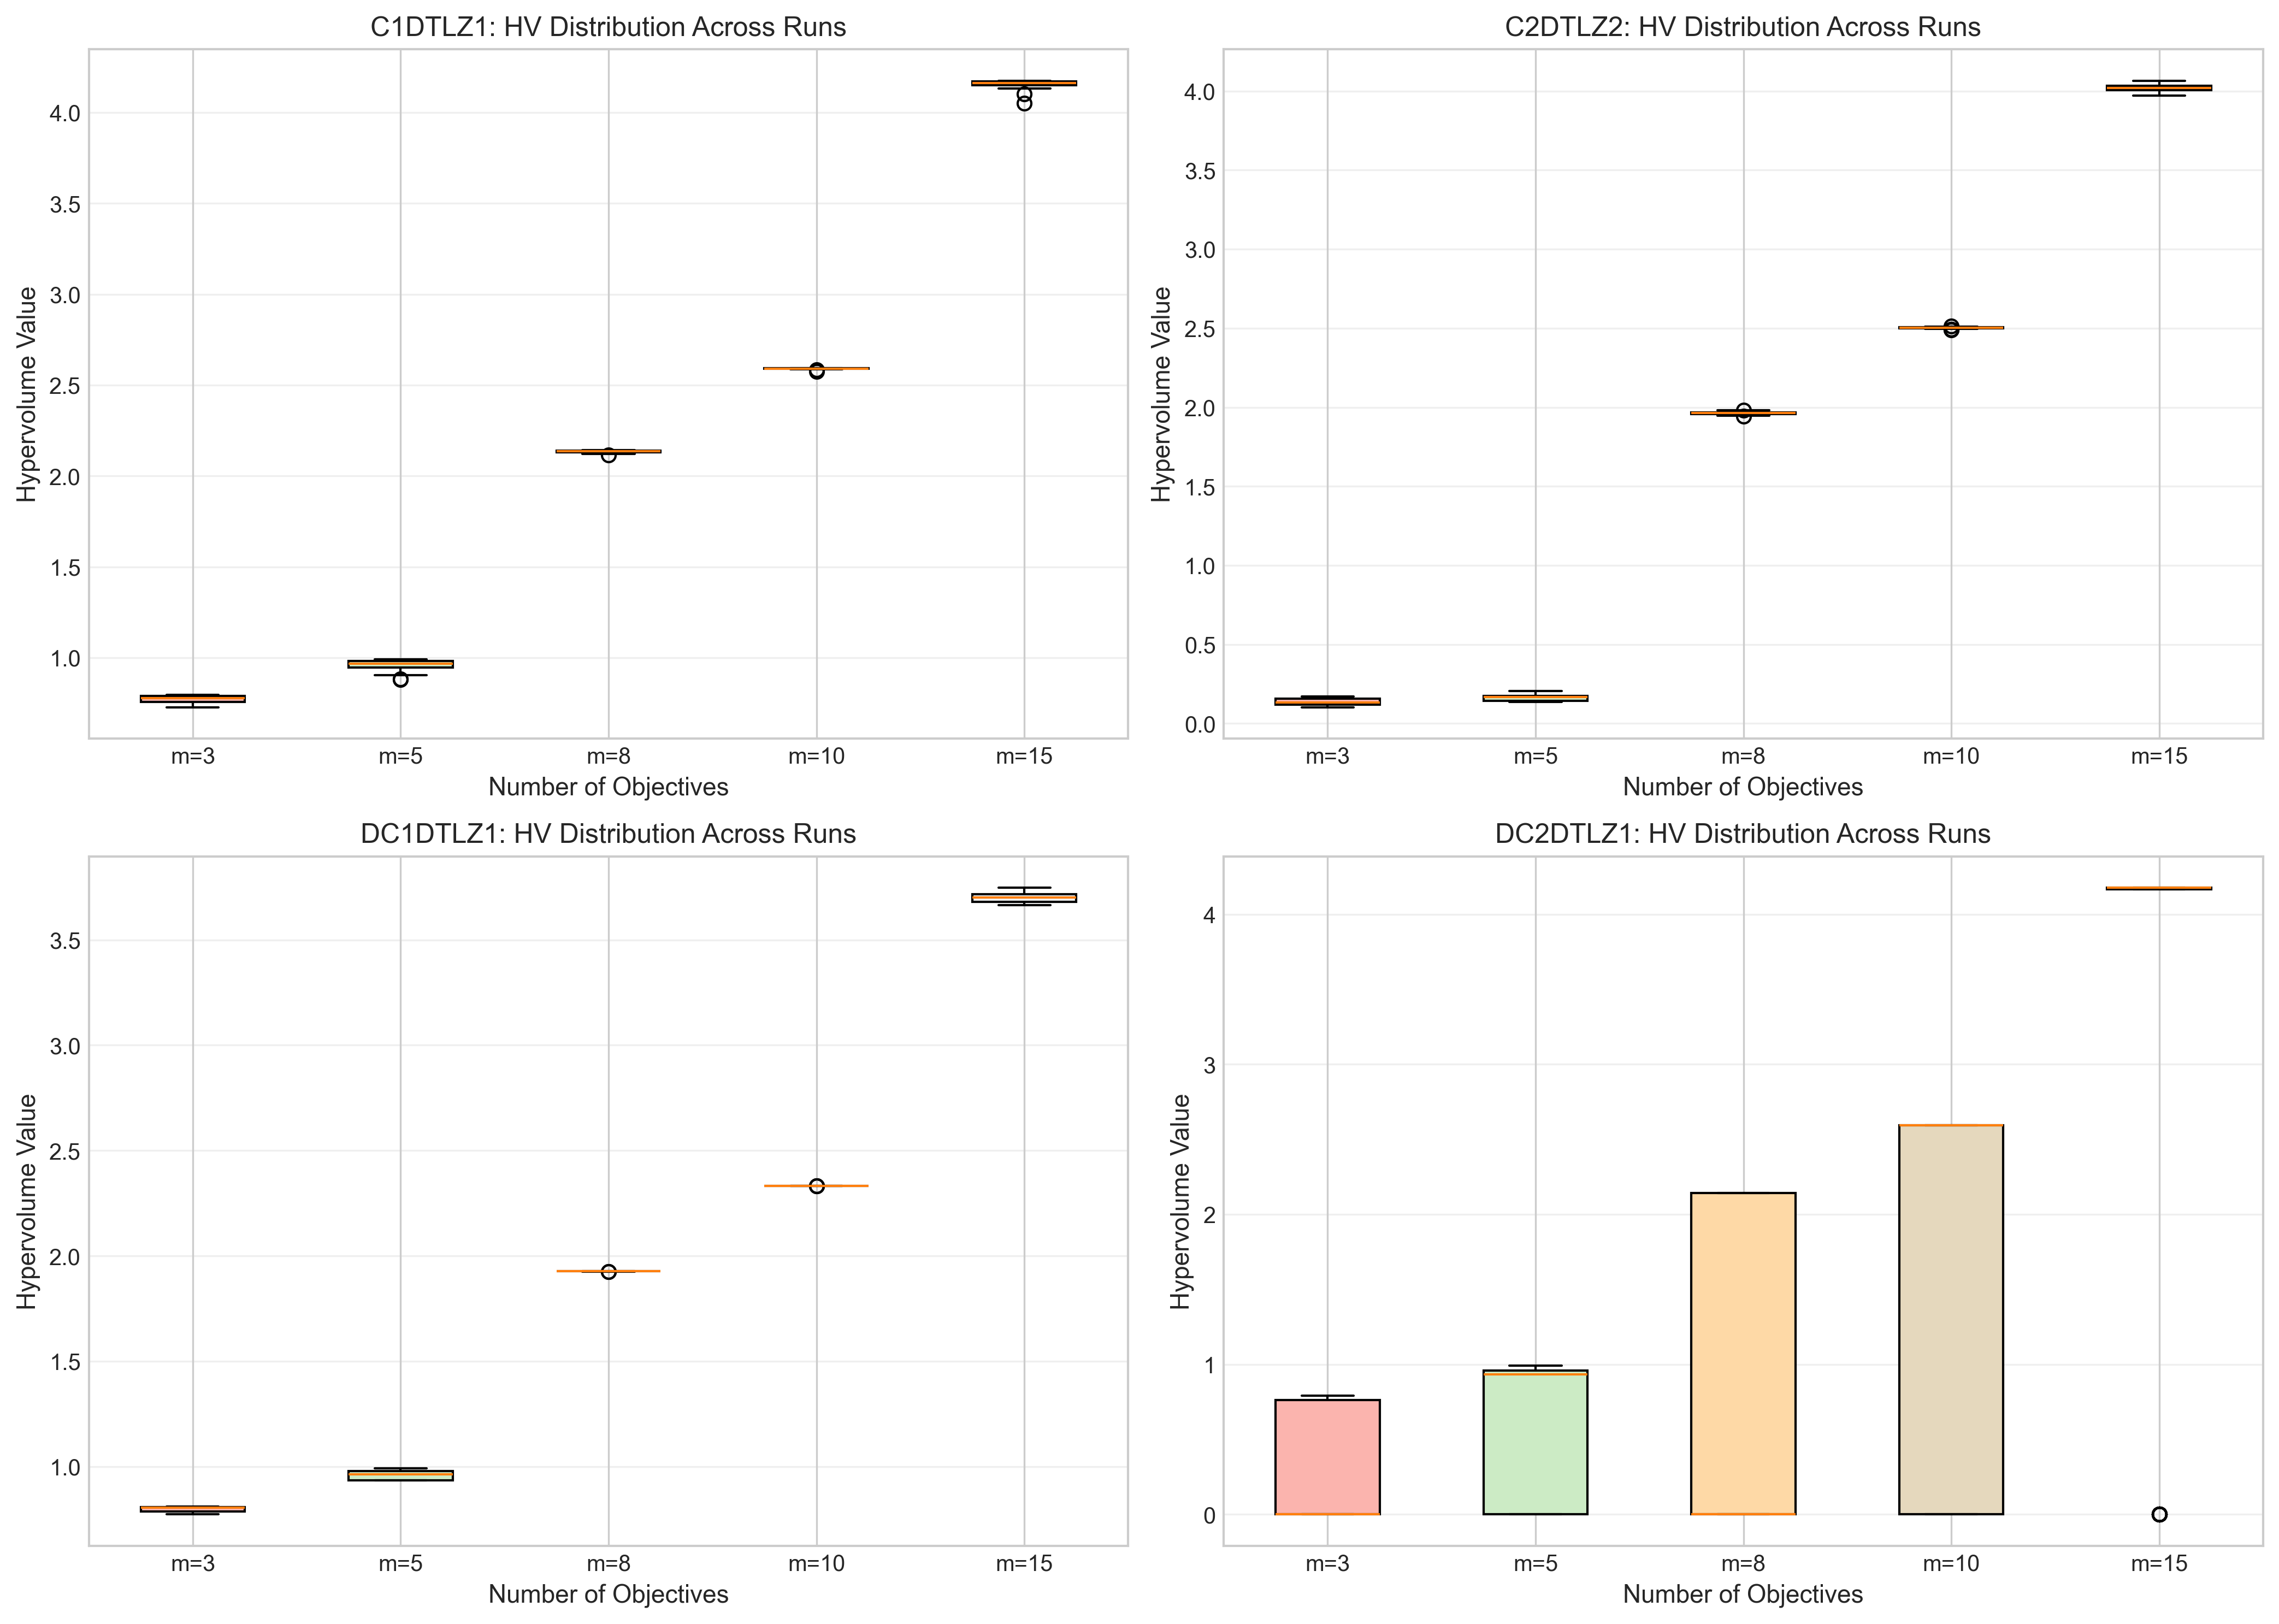
\includegraphics[width=0.85\textwidth]{runs_distribution_hv.png}
    \caption{HV Distribution across runs}
\end{figure}

\begin{figure}[h!]
    \centering
    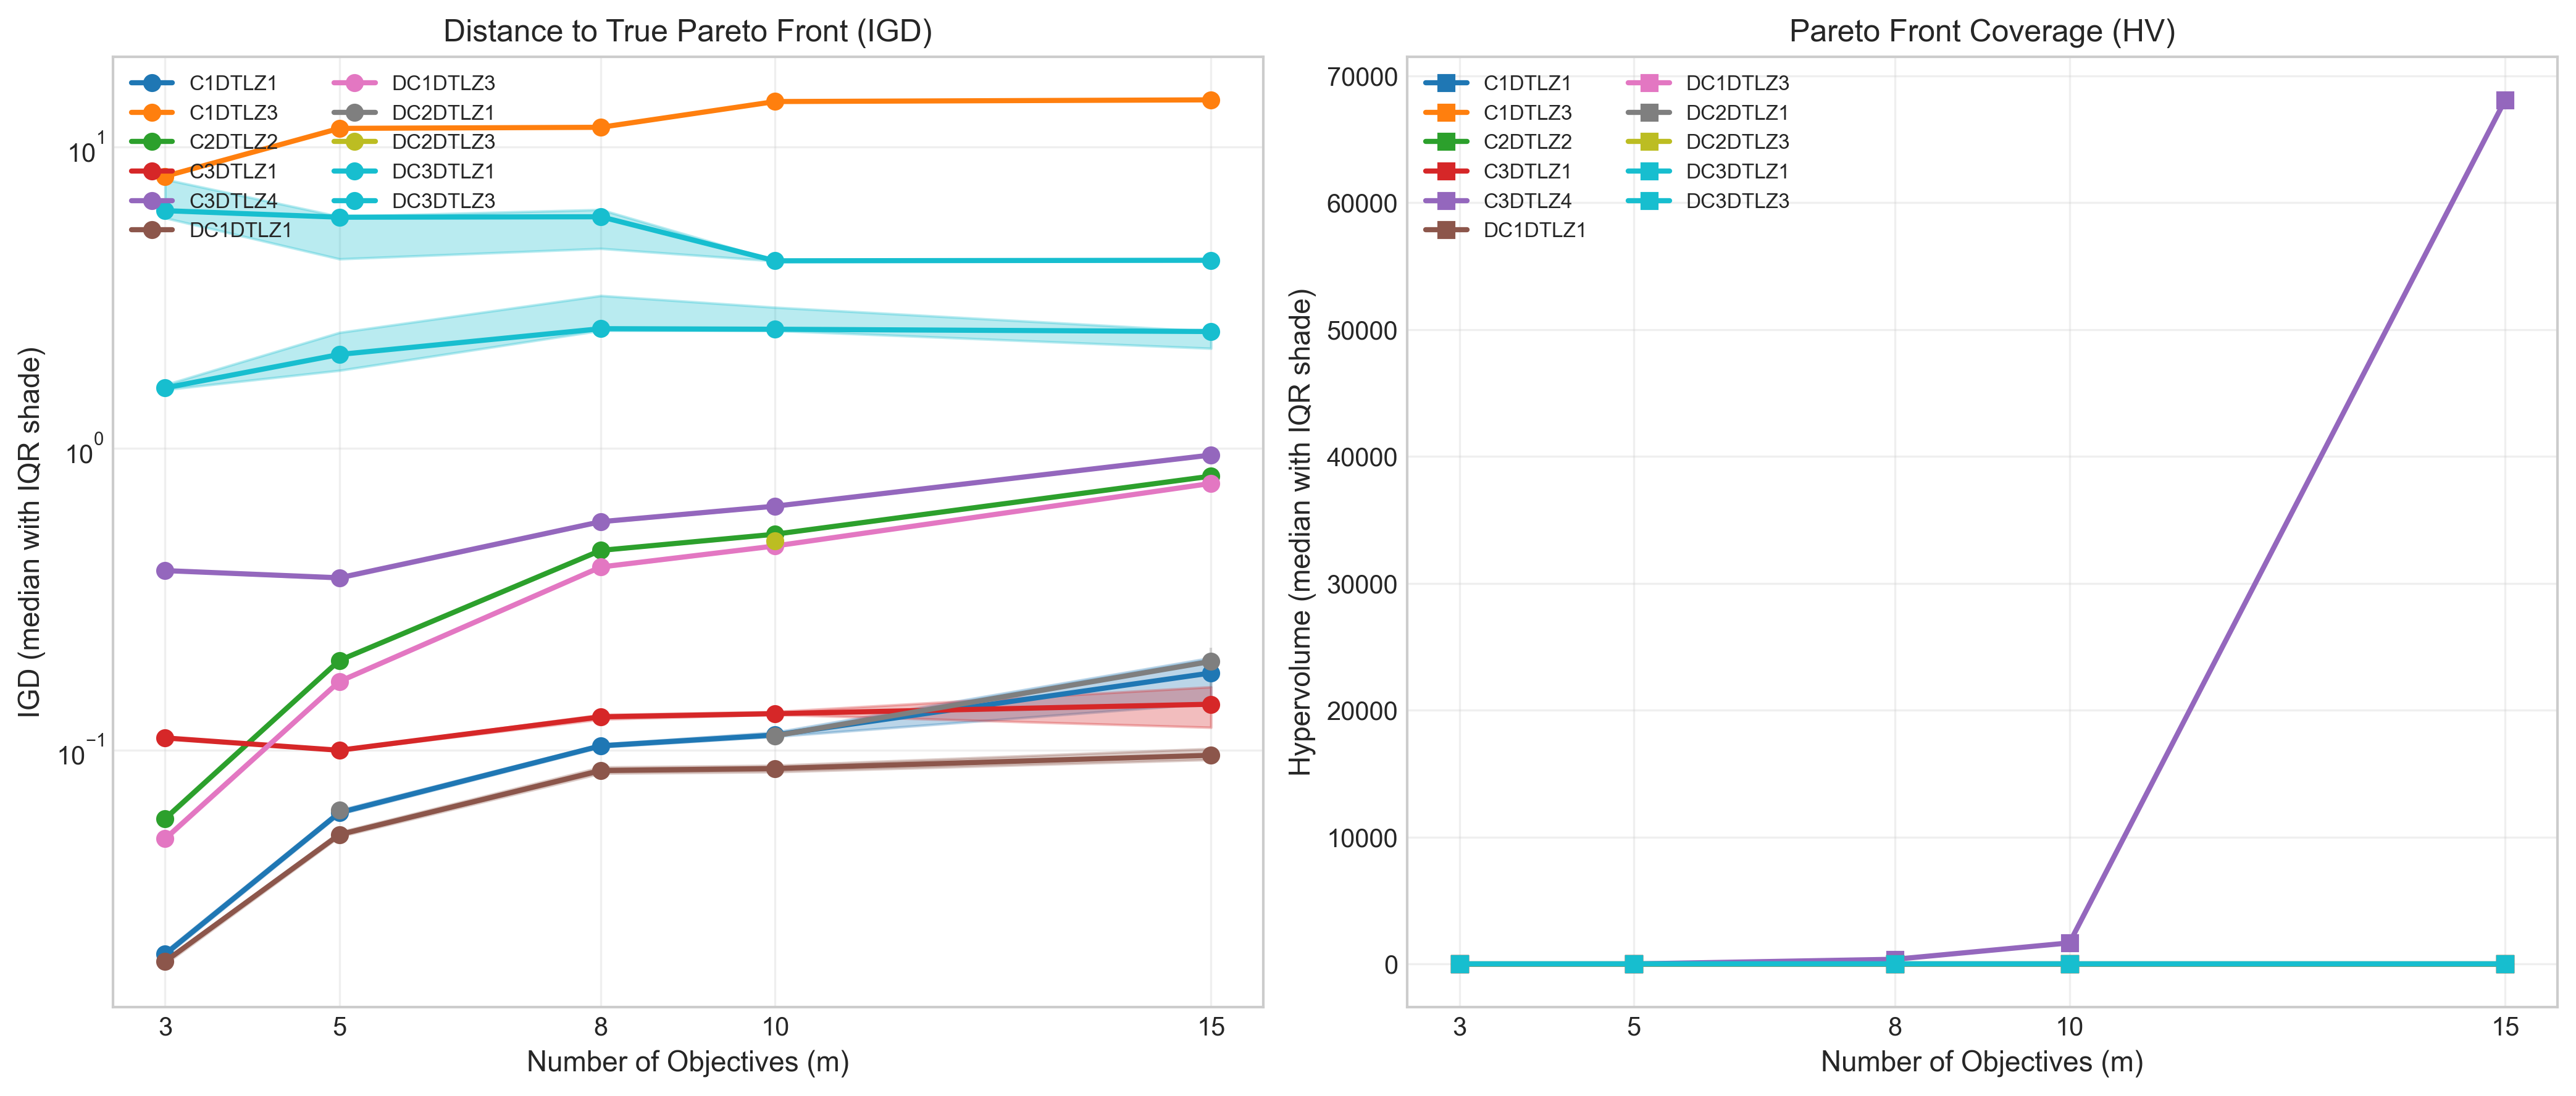
\includegraphics[width=0.85\textwidth]{convergence_profile.png}
    \caption{Convergence Profile}
\end{figure}

\begin{figure}[h!]
    \centering
    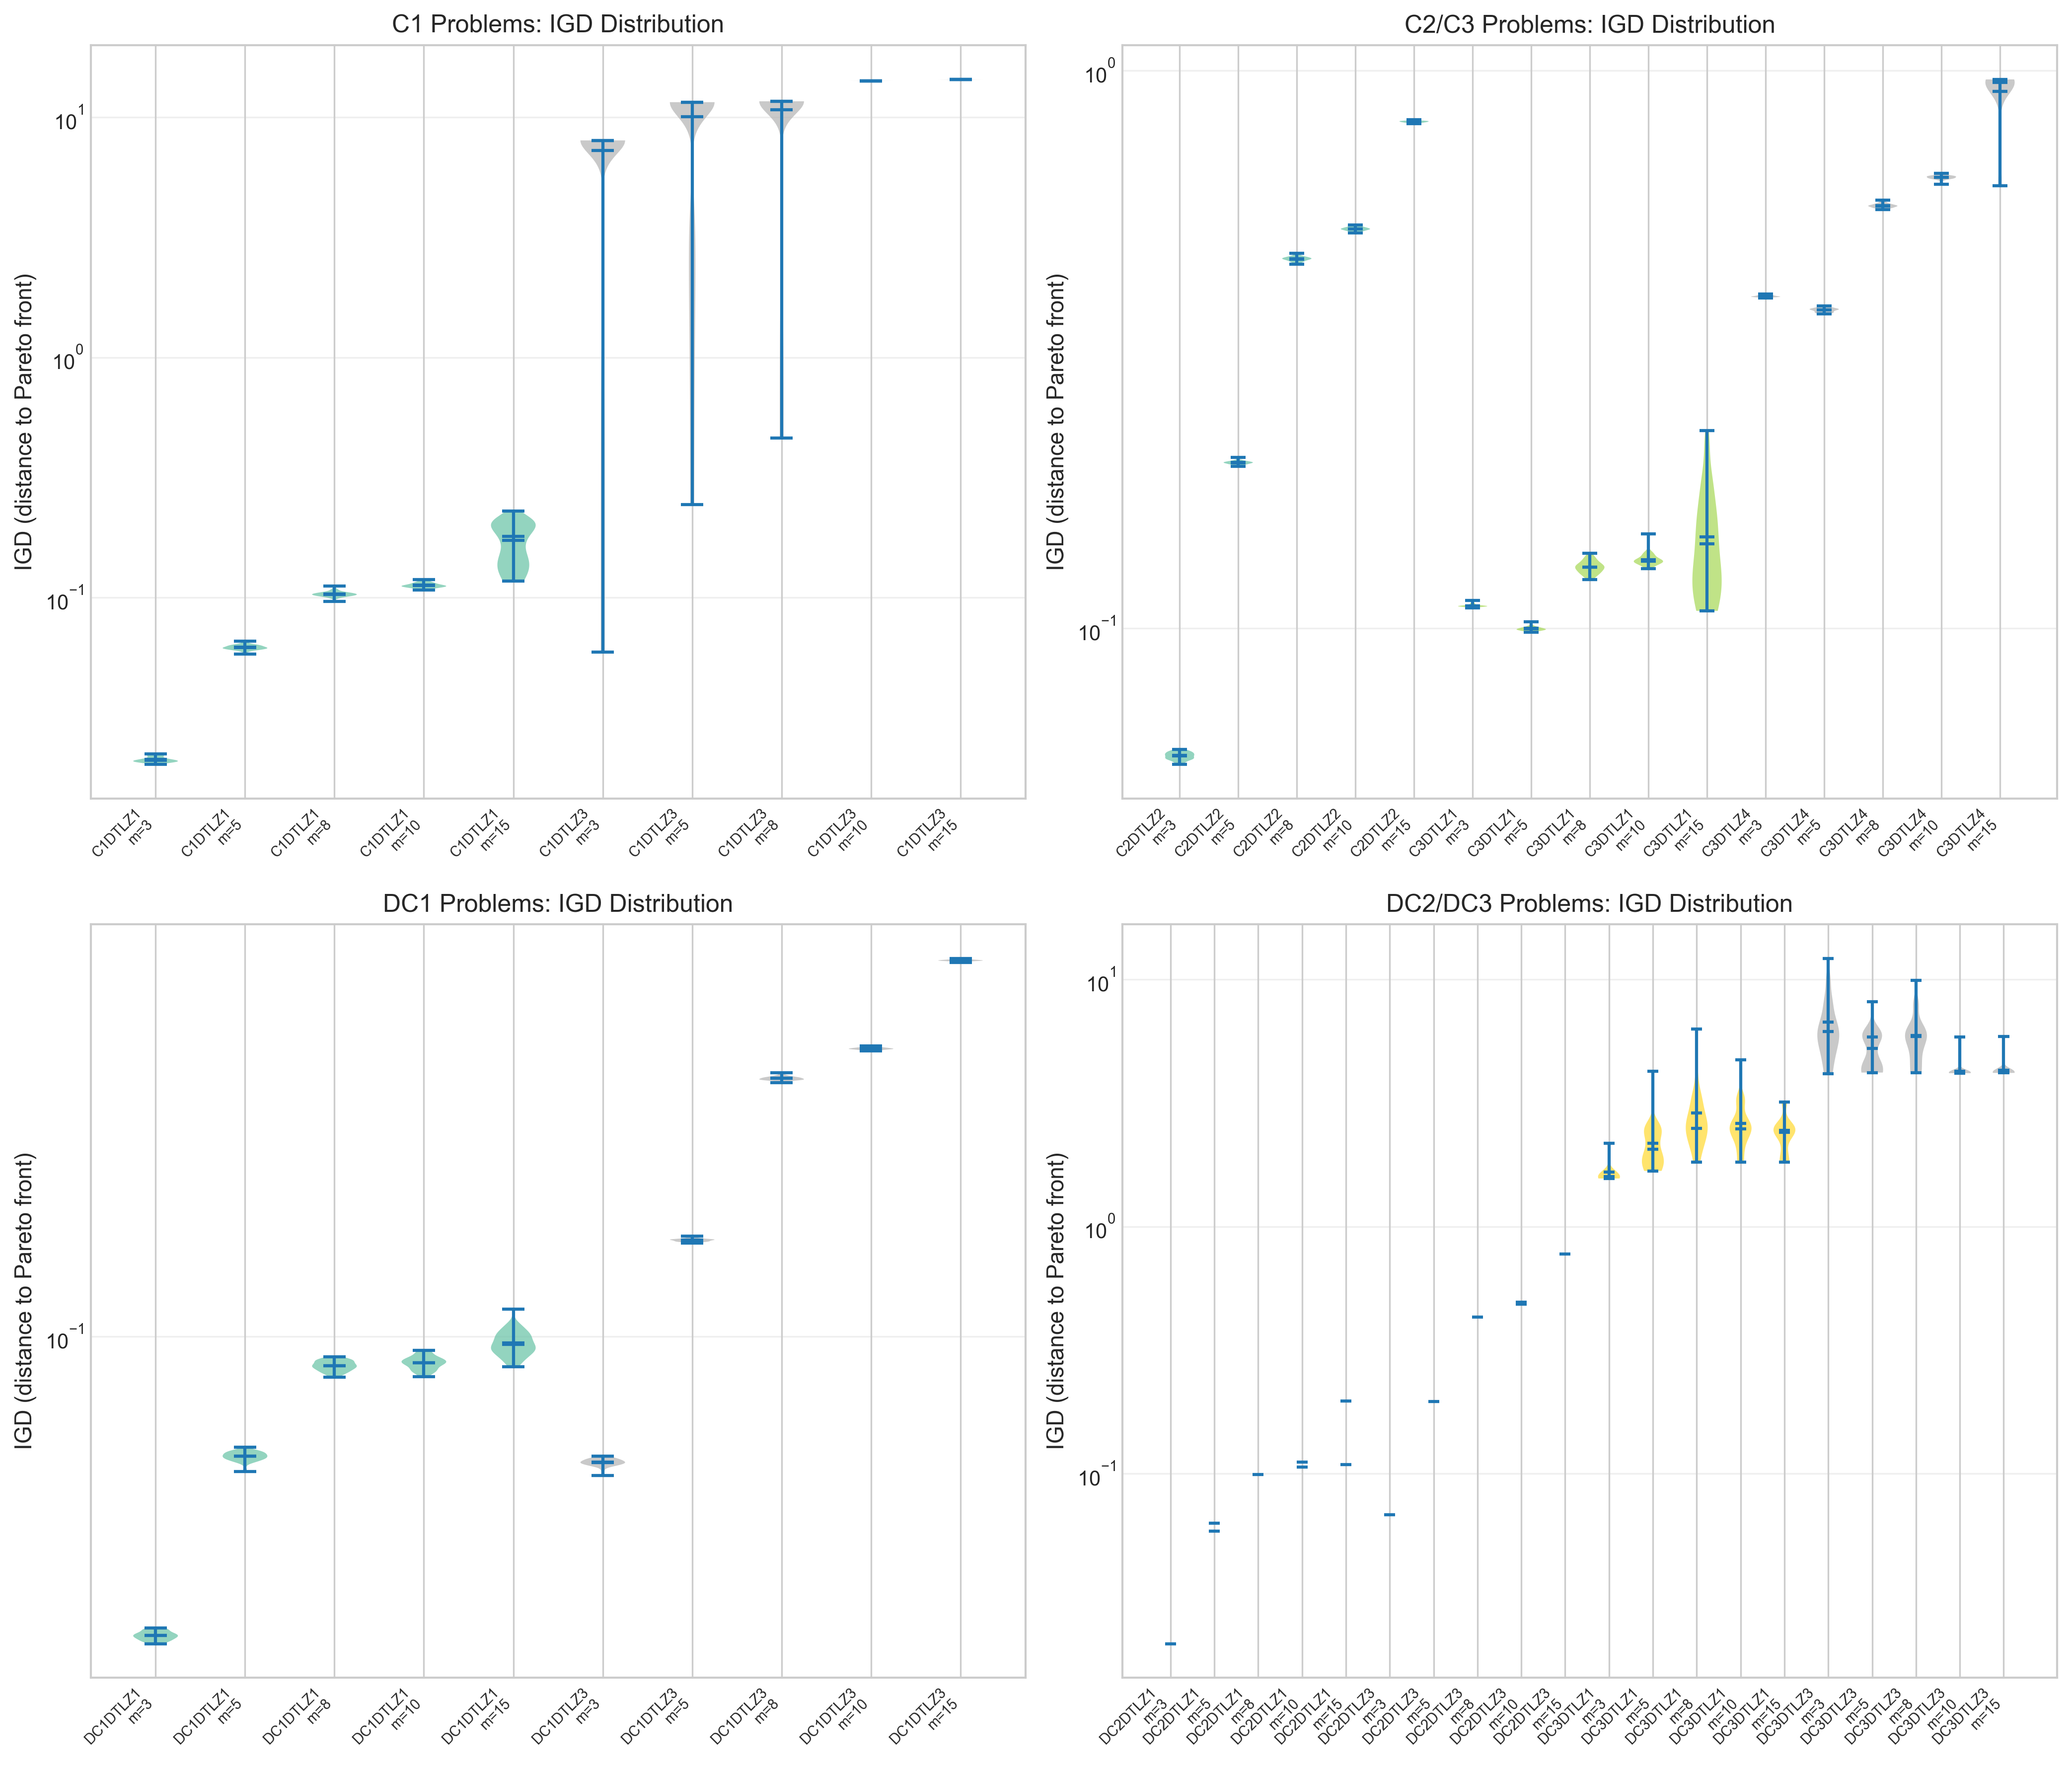
\includegraphics[width=0.75\textwidth]{igd_distribution_violin.png}
    \caption{IGD Distribution for each problem class}
\end{figure}

\begin{figure}[h!]
    \centering
    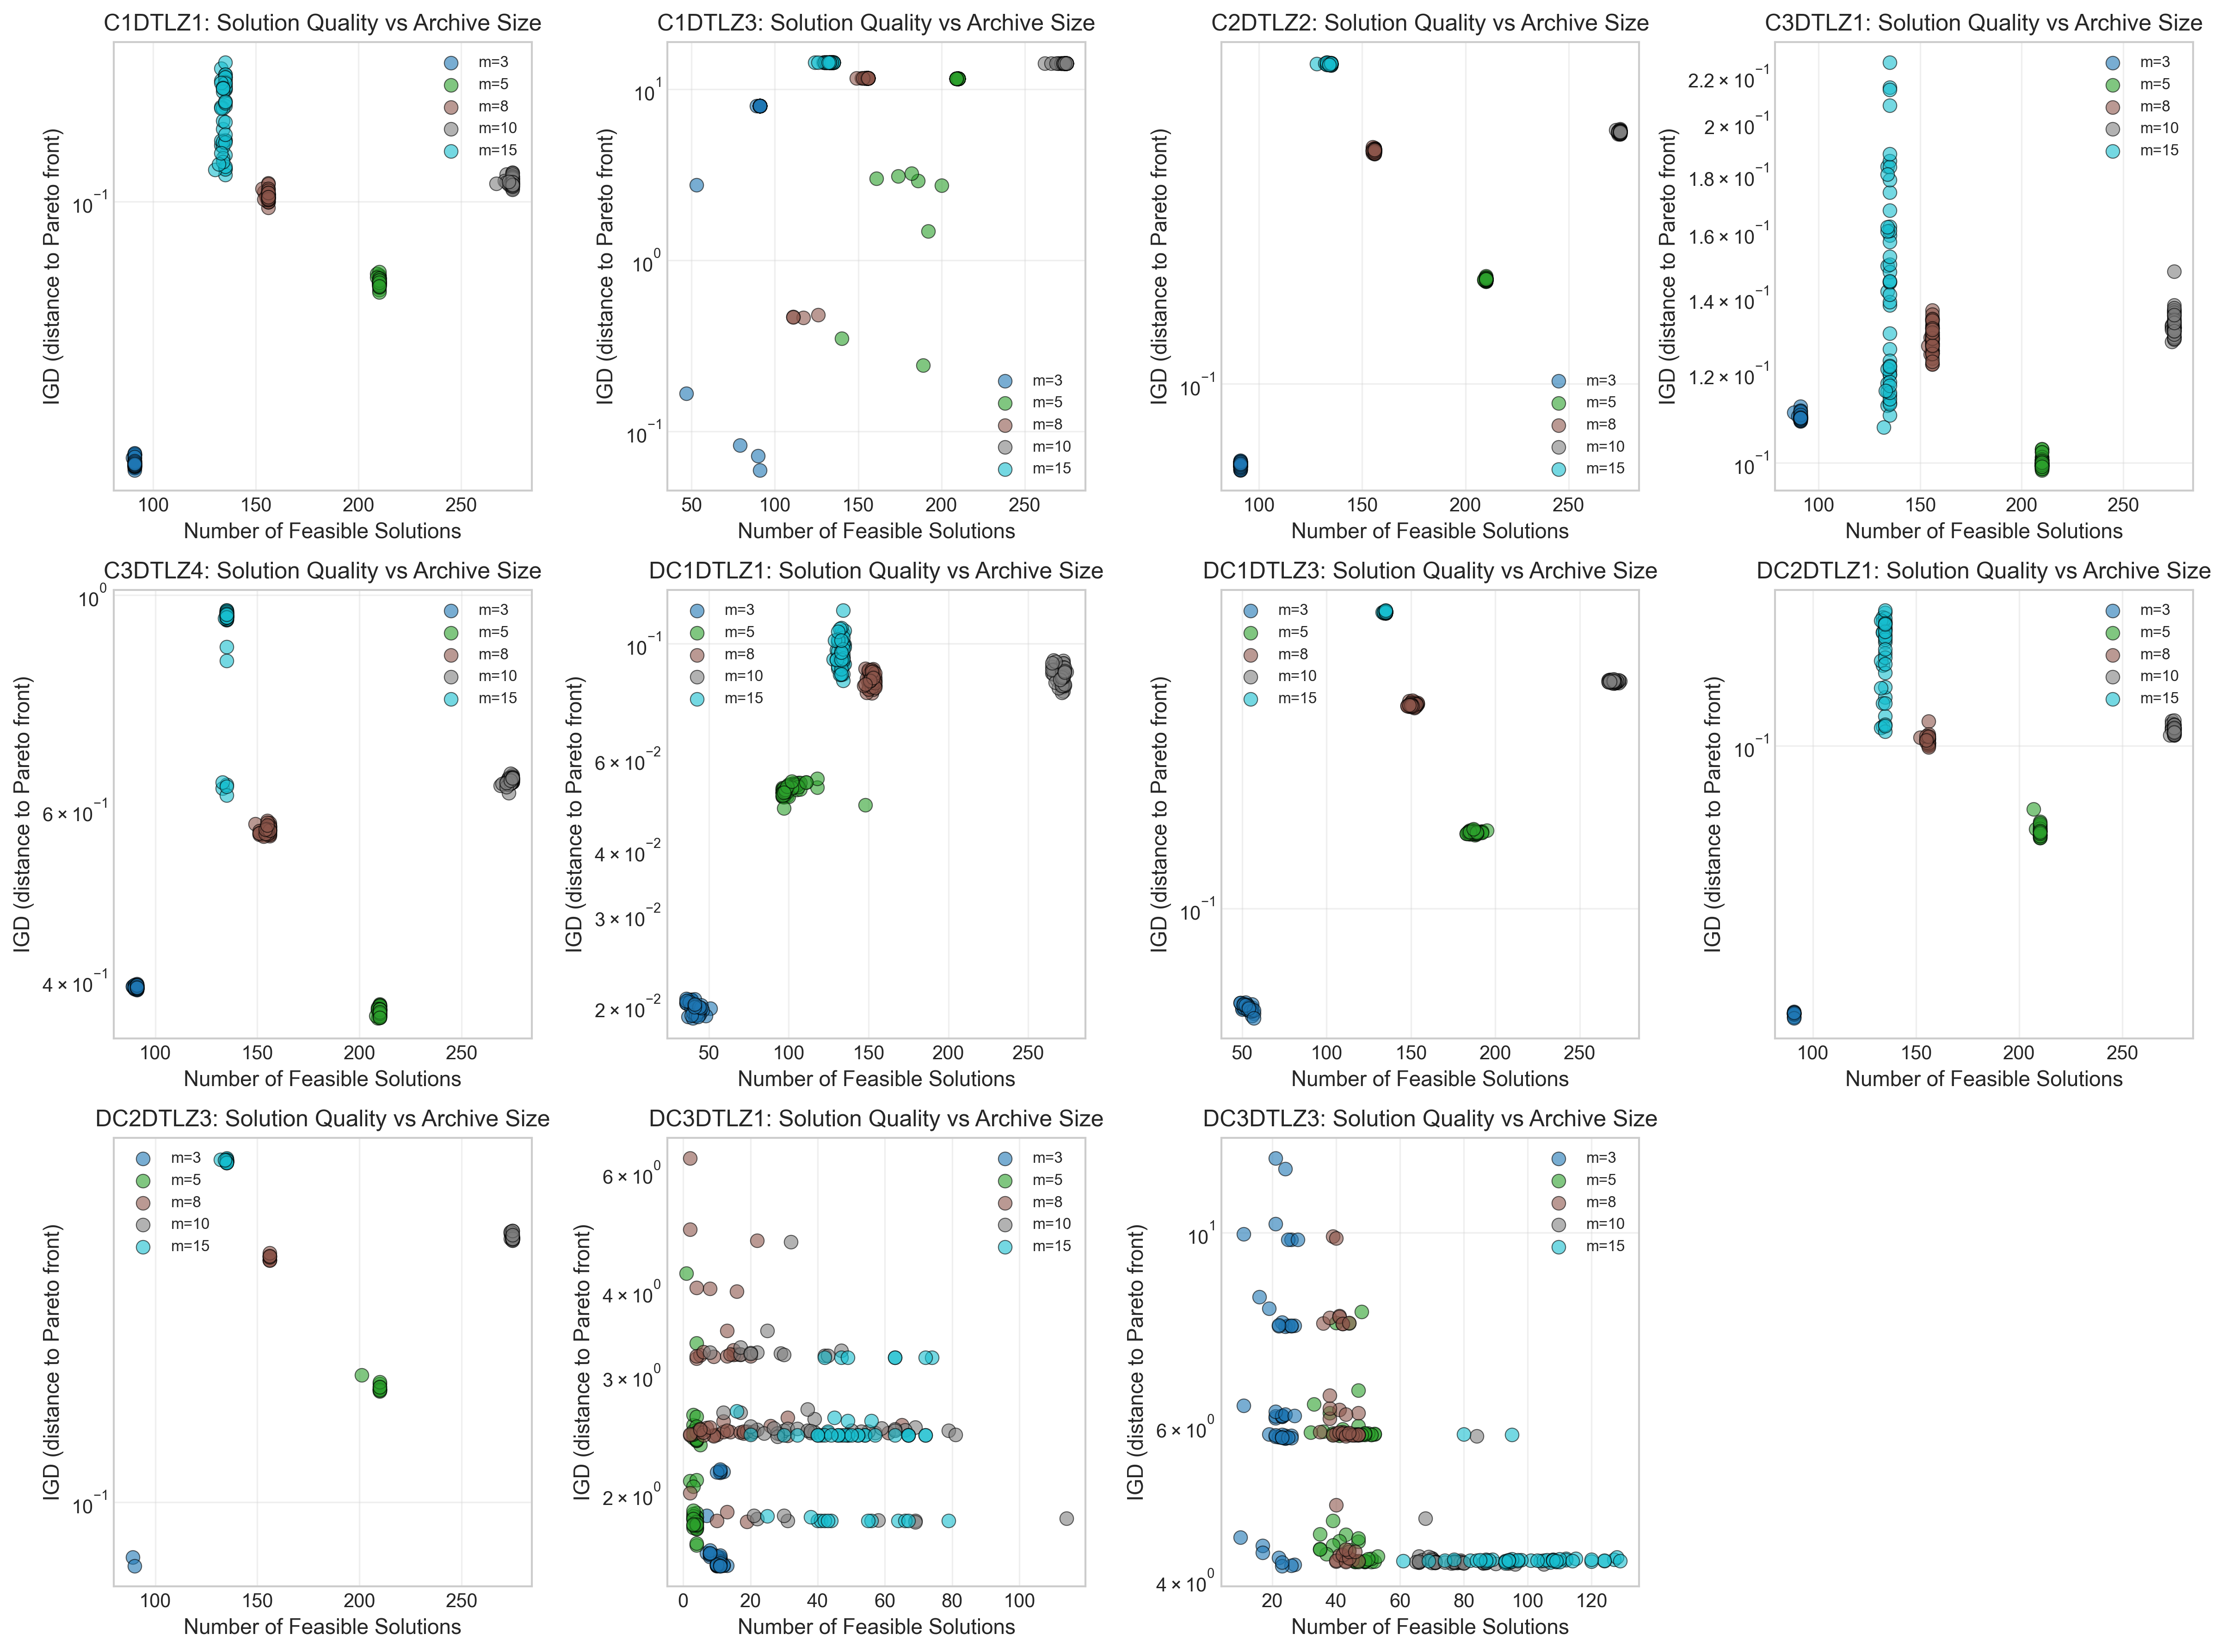
\includegraphics[width=0.85\textwidth]{igd_vs_feasible_solutions.png}
    \caption{IGD vs Number of feasible solutions}
\end{figure}

\begin{figure}[h!]
    \centering
    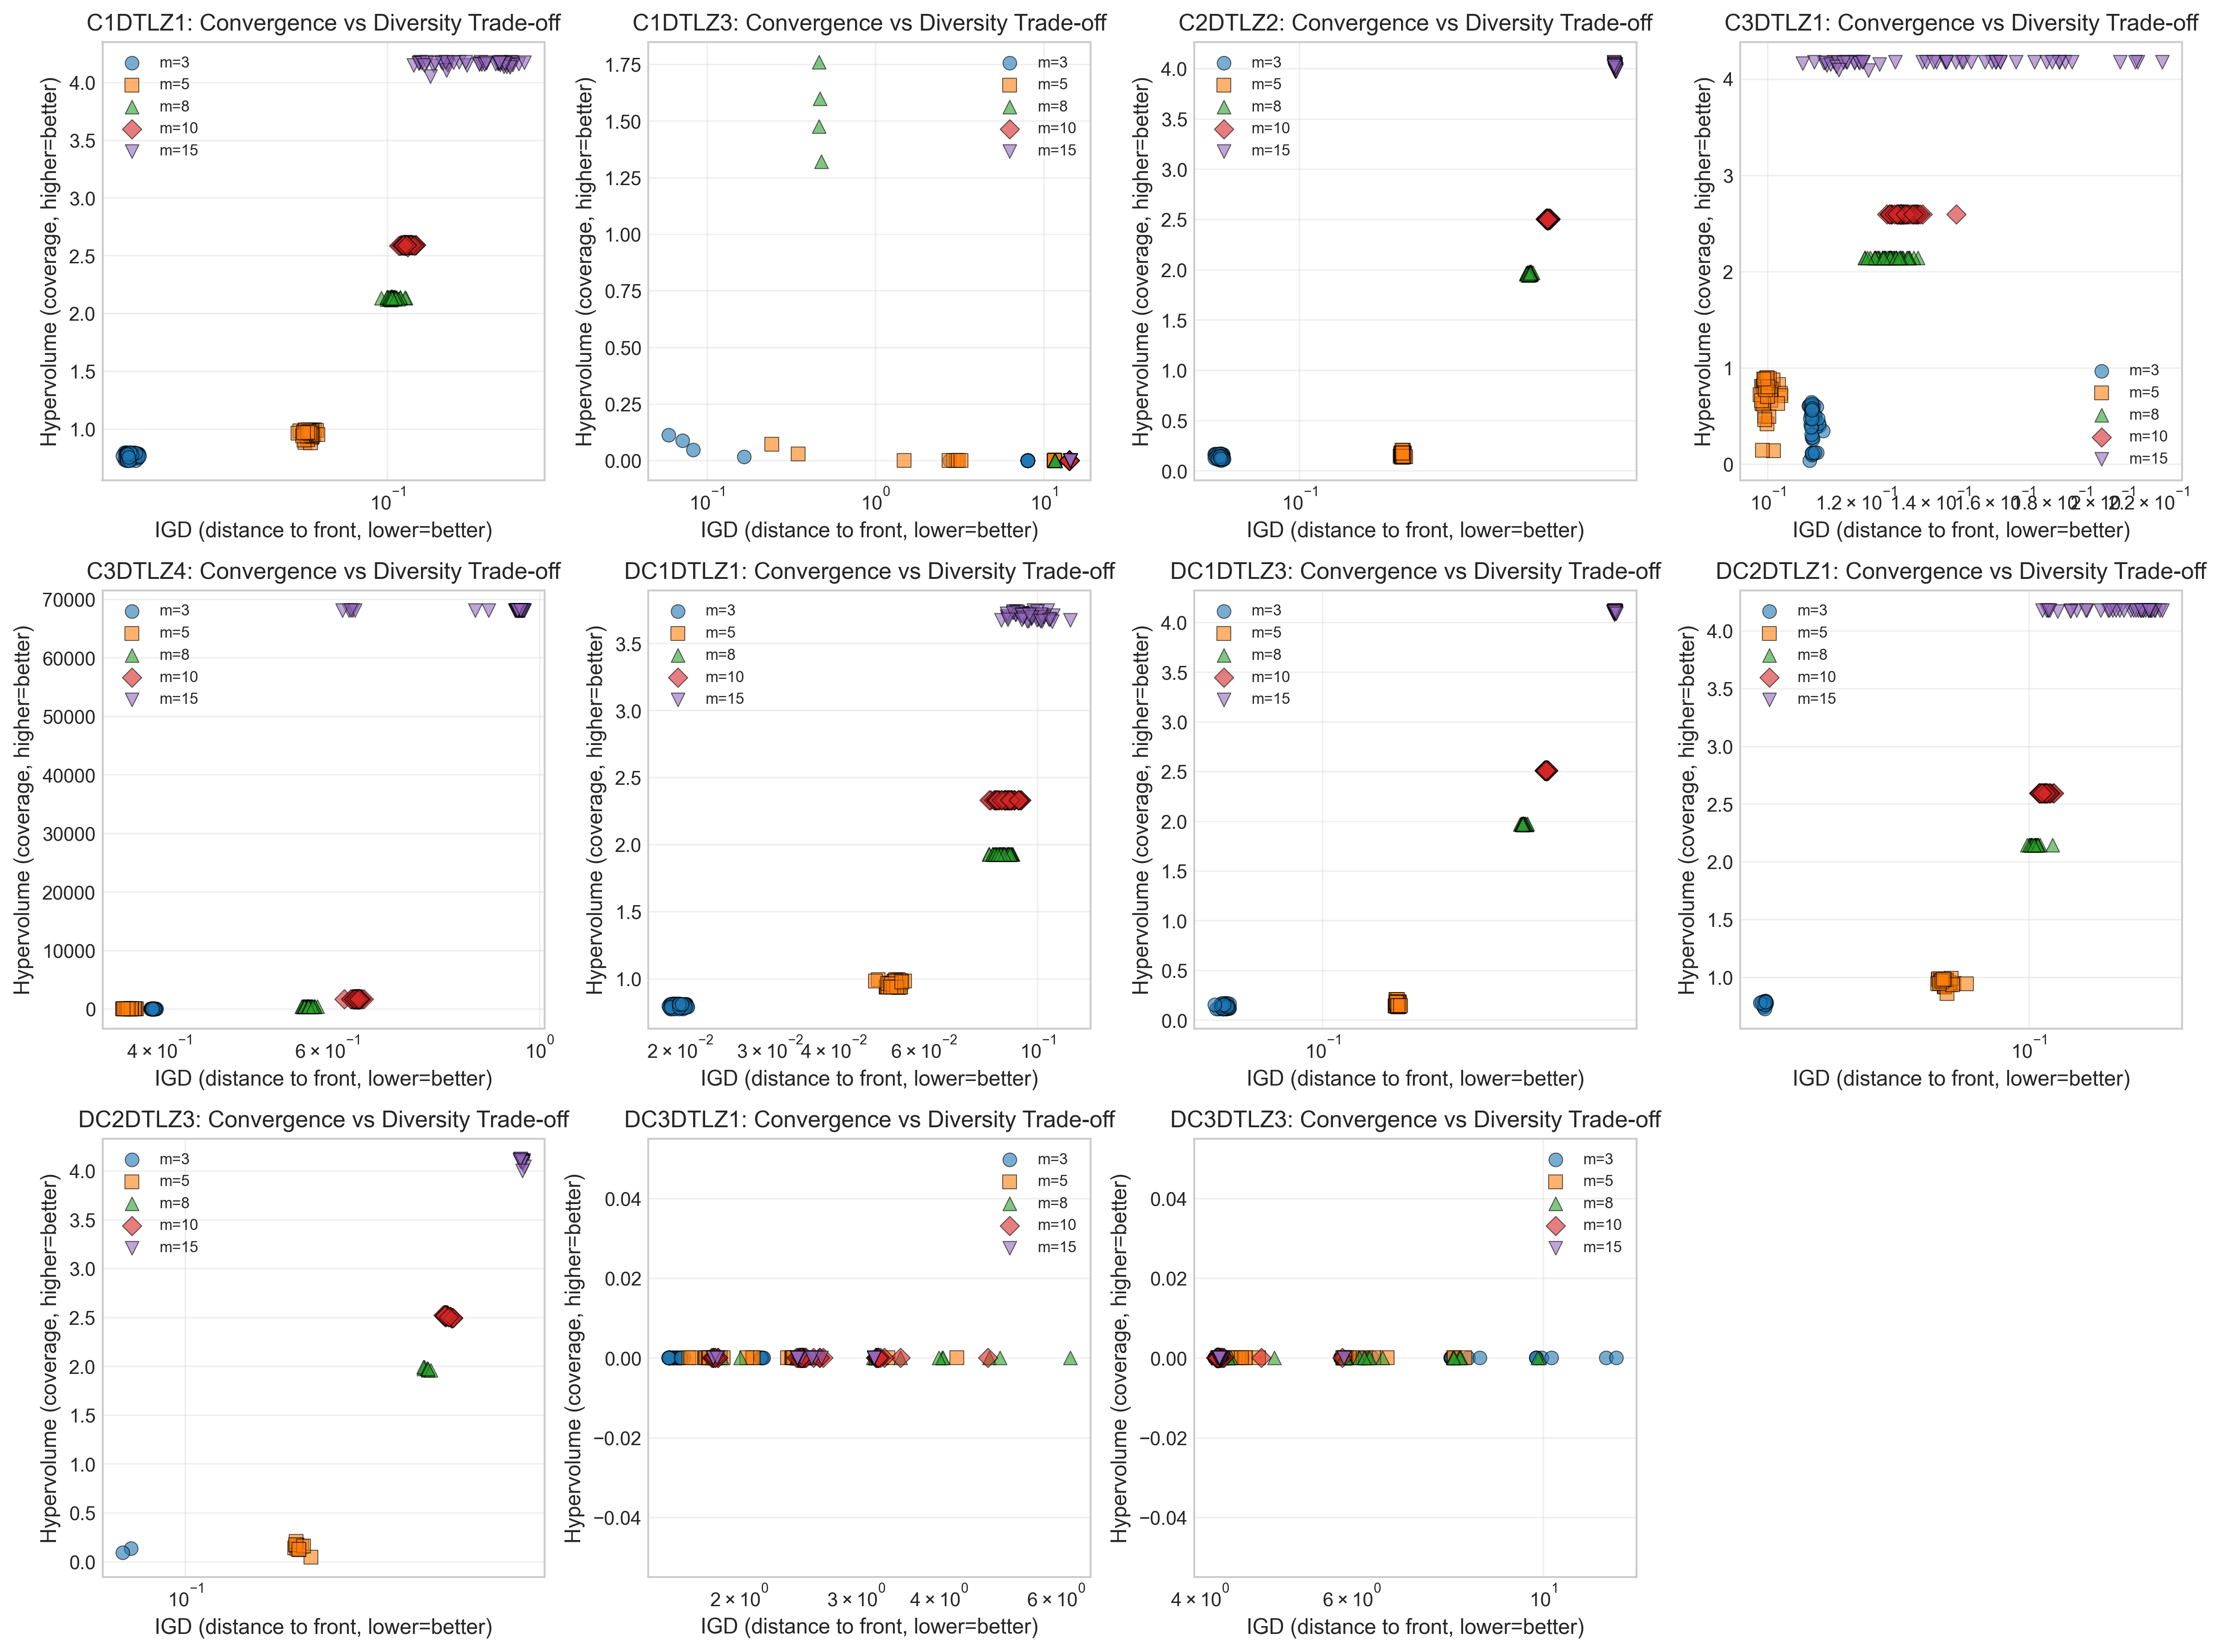
\includegraphics[width=0.85\textwidth]{igd_vs_hv_tradeoff.png}
    \caption{IGD vs HV tradeoff}
\end{figure}

\begin{figure}[h!]
    \centering
    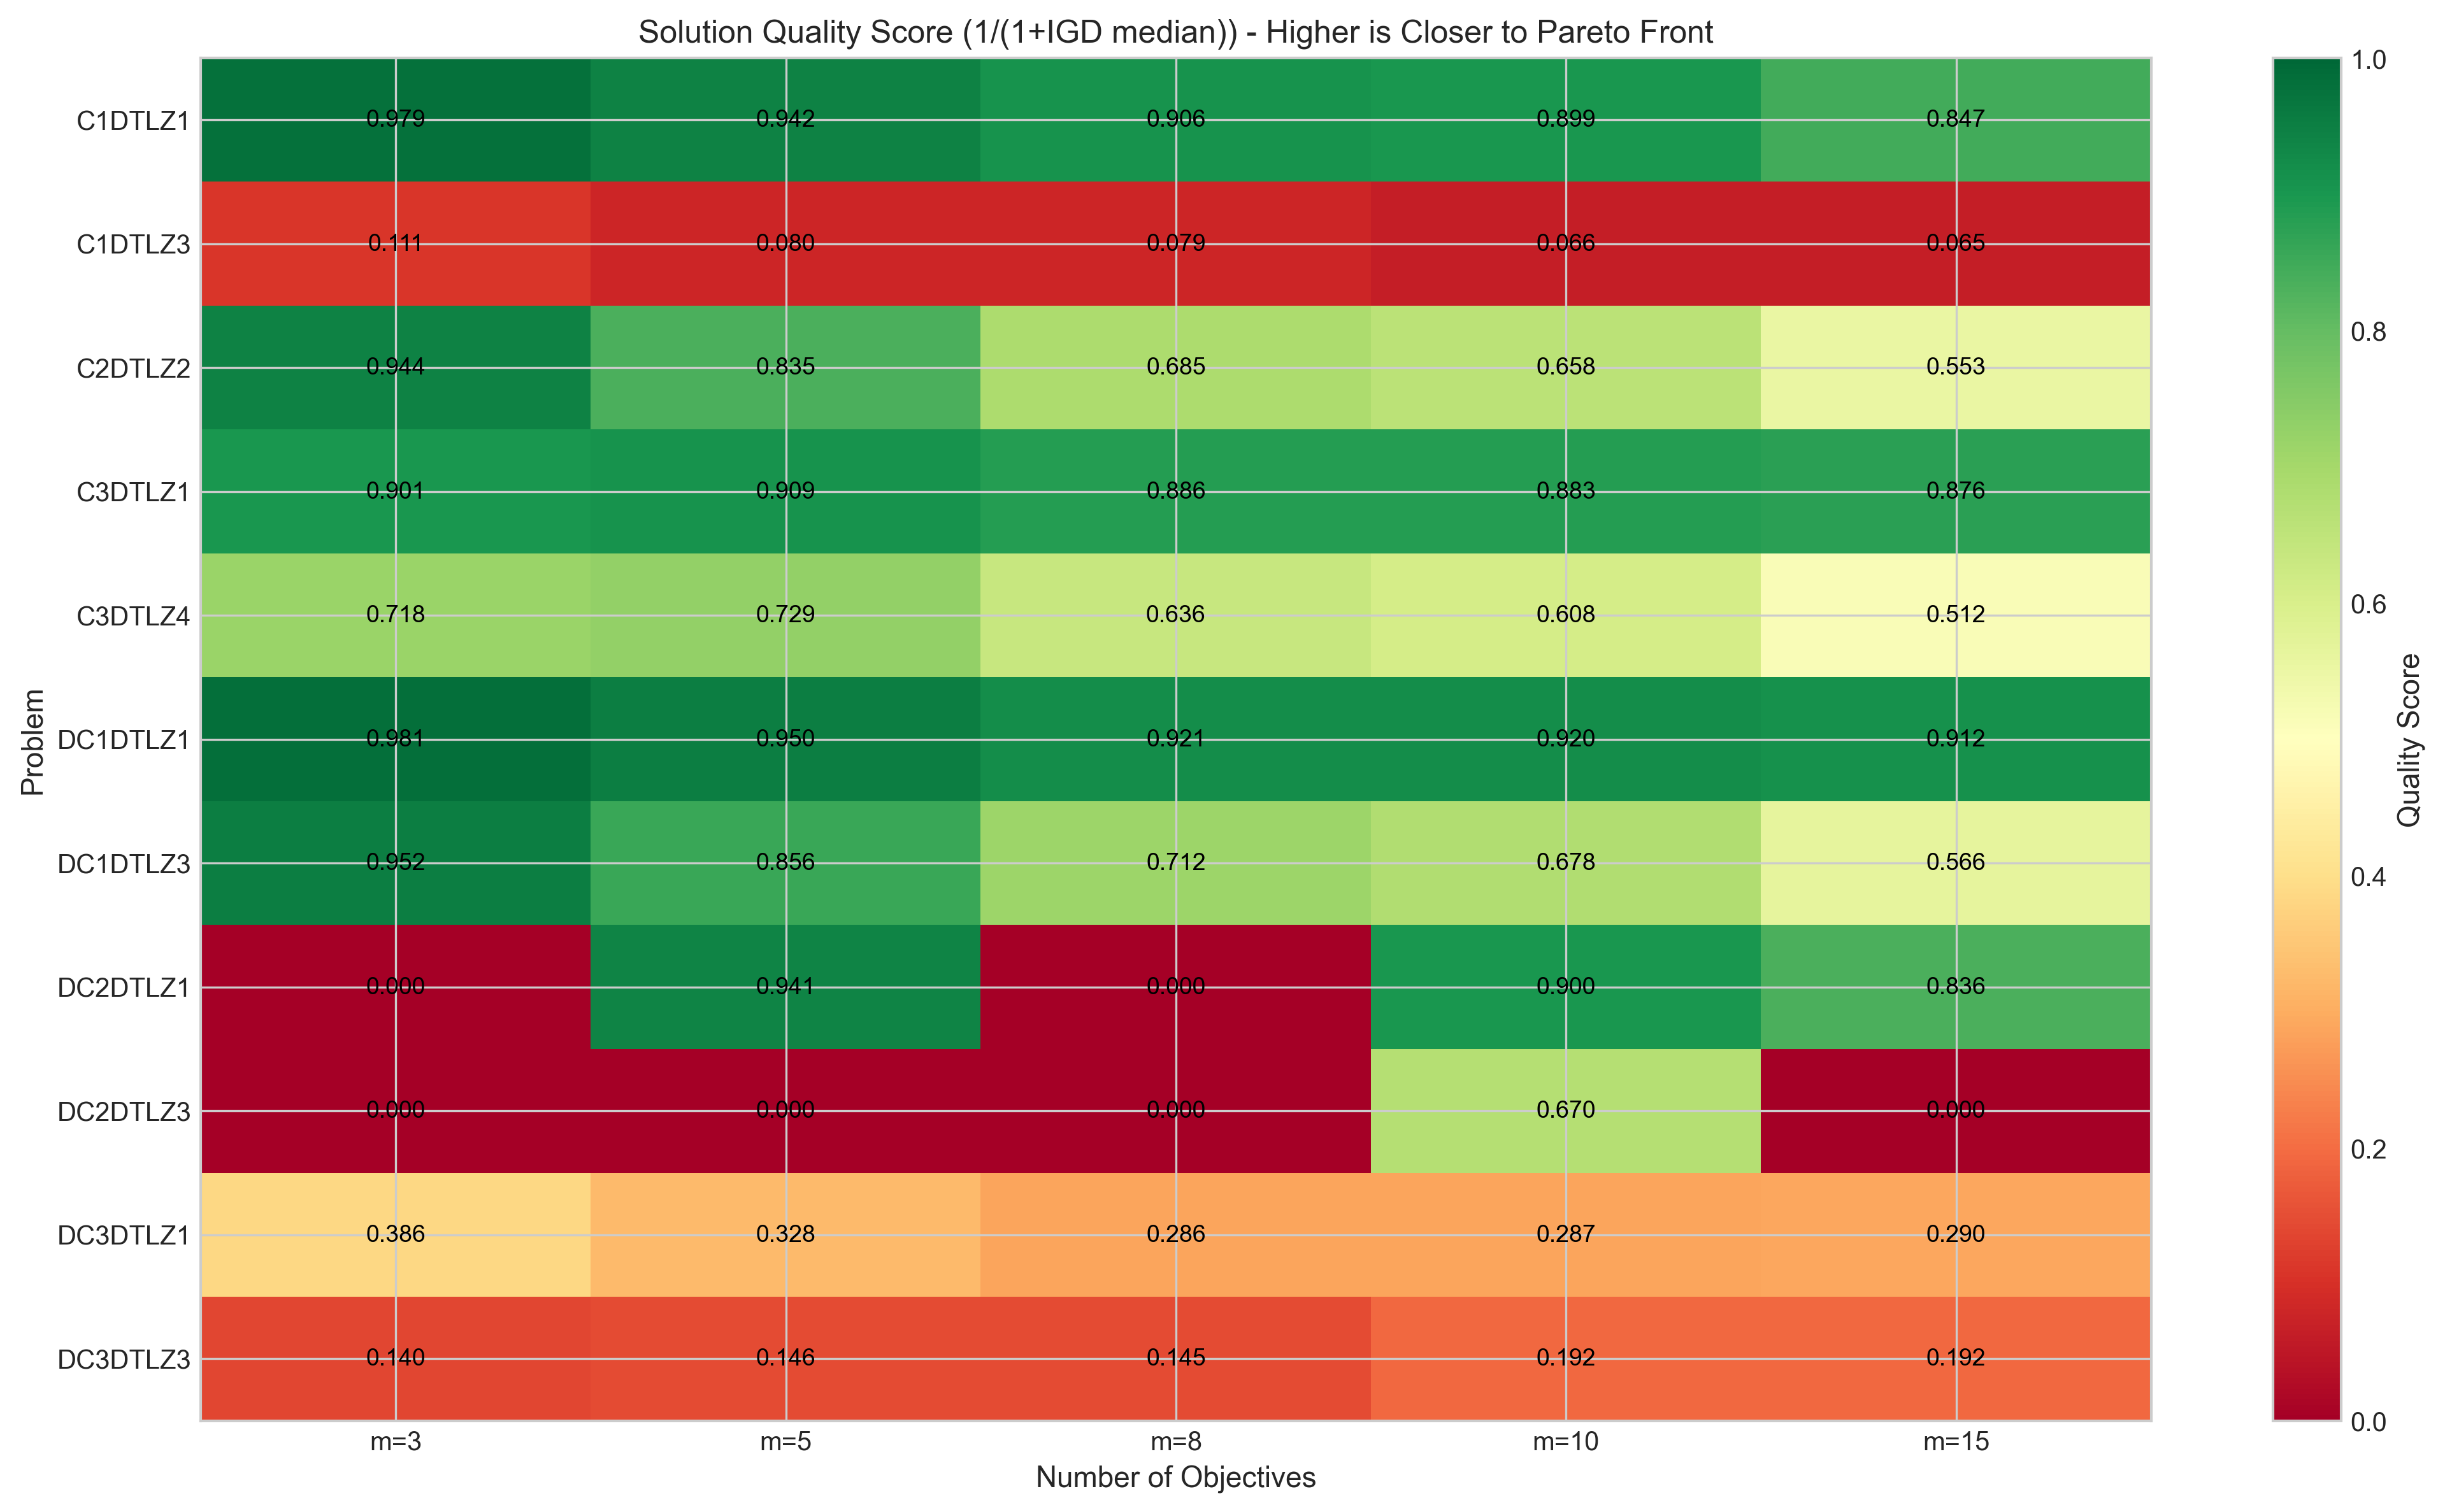
\includegraphics[width=0.85\textwidth]{solution_quality_heatmap.png}
    \caption{Solution Quality Heatmap}
\end{figure}

\begin{figure}[h!]
    \centering
    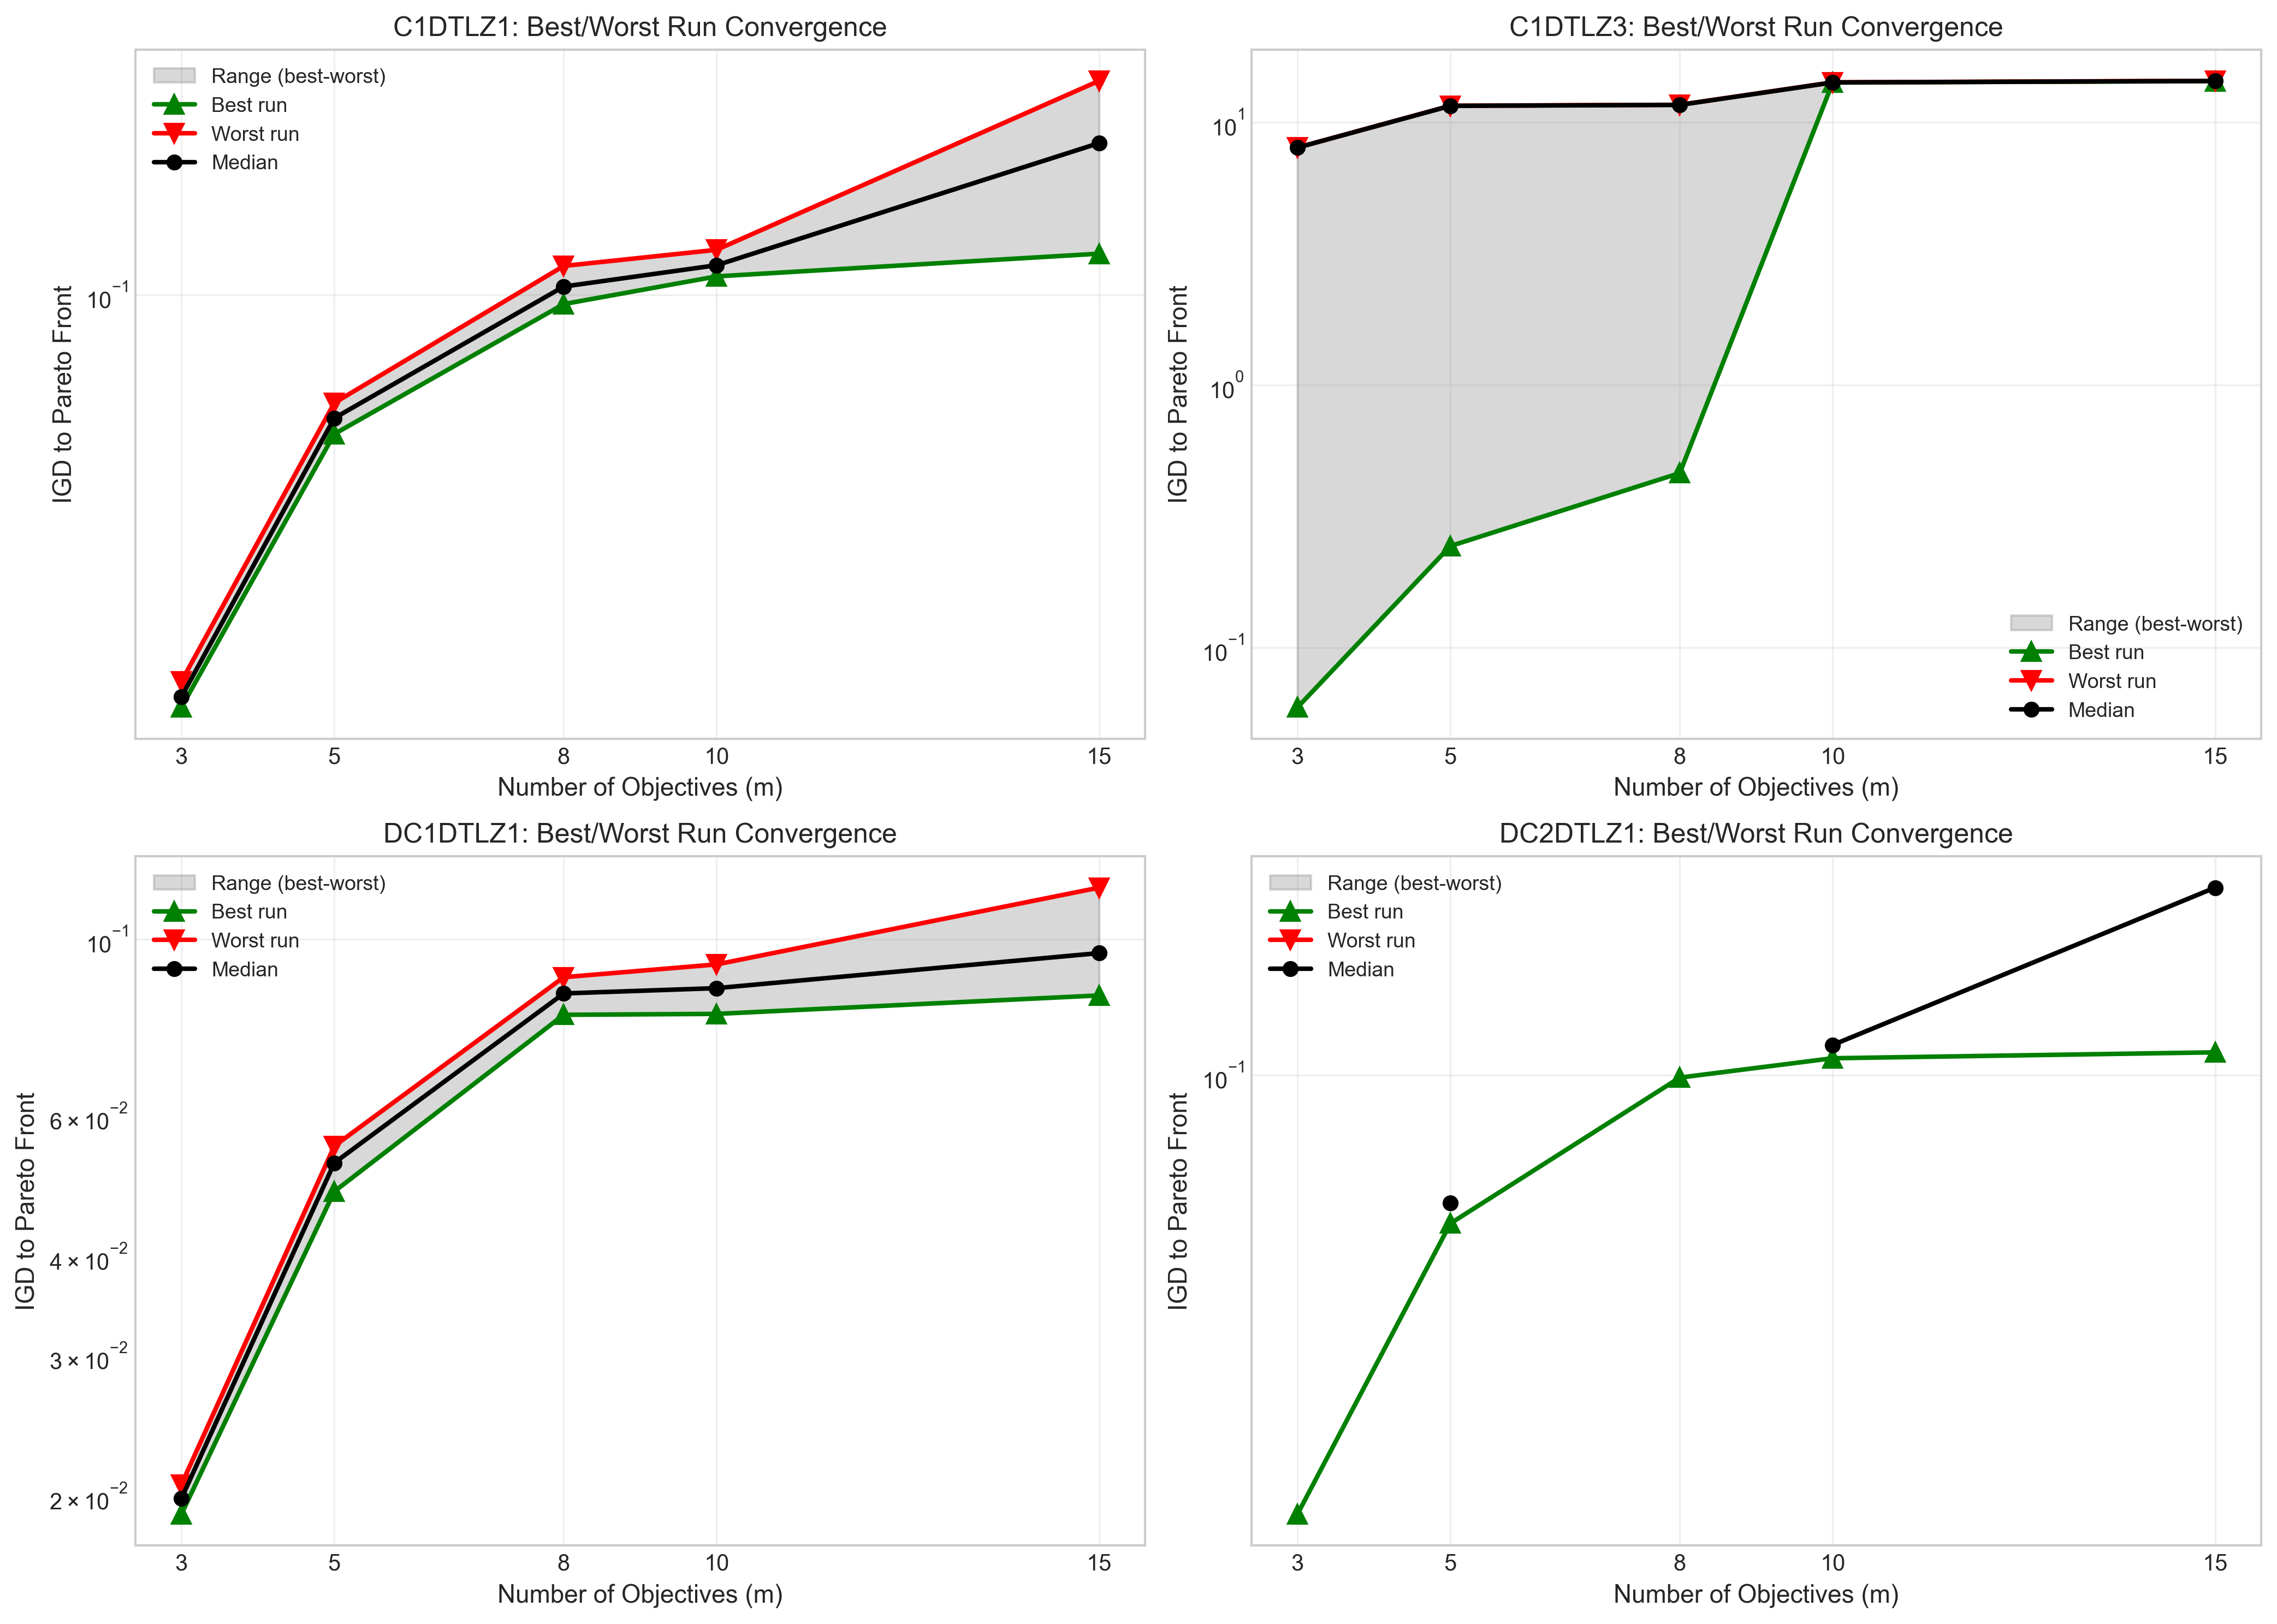
\includegraphics[width=0.85\textwidth]{best_worst_runs.png}
    \caption{Best Worst Runs}
\end{figure}


\begin{figure}[h!]
    \centering
    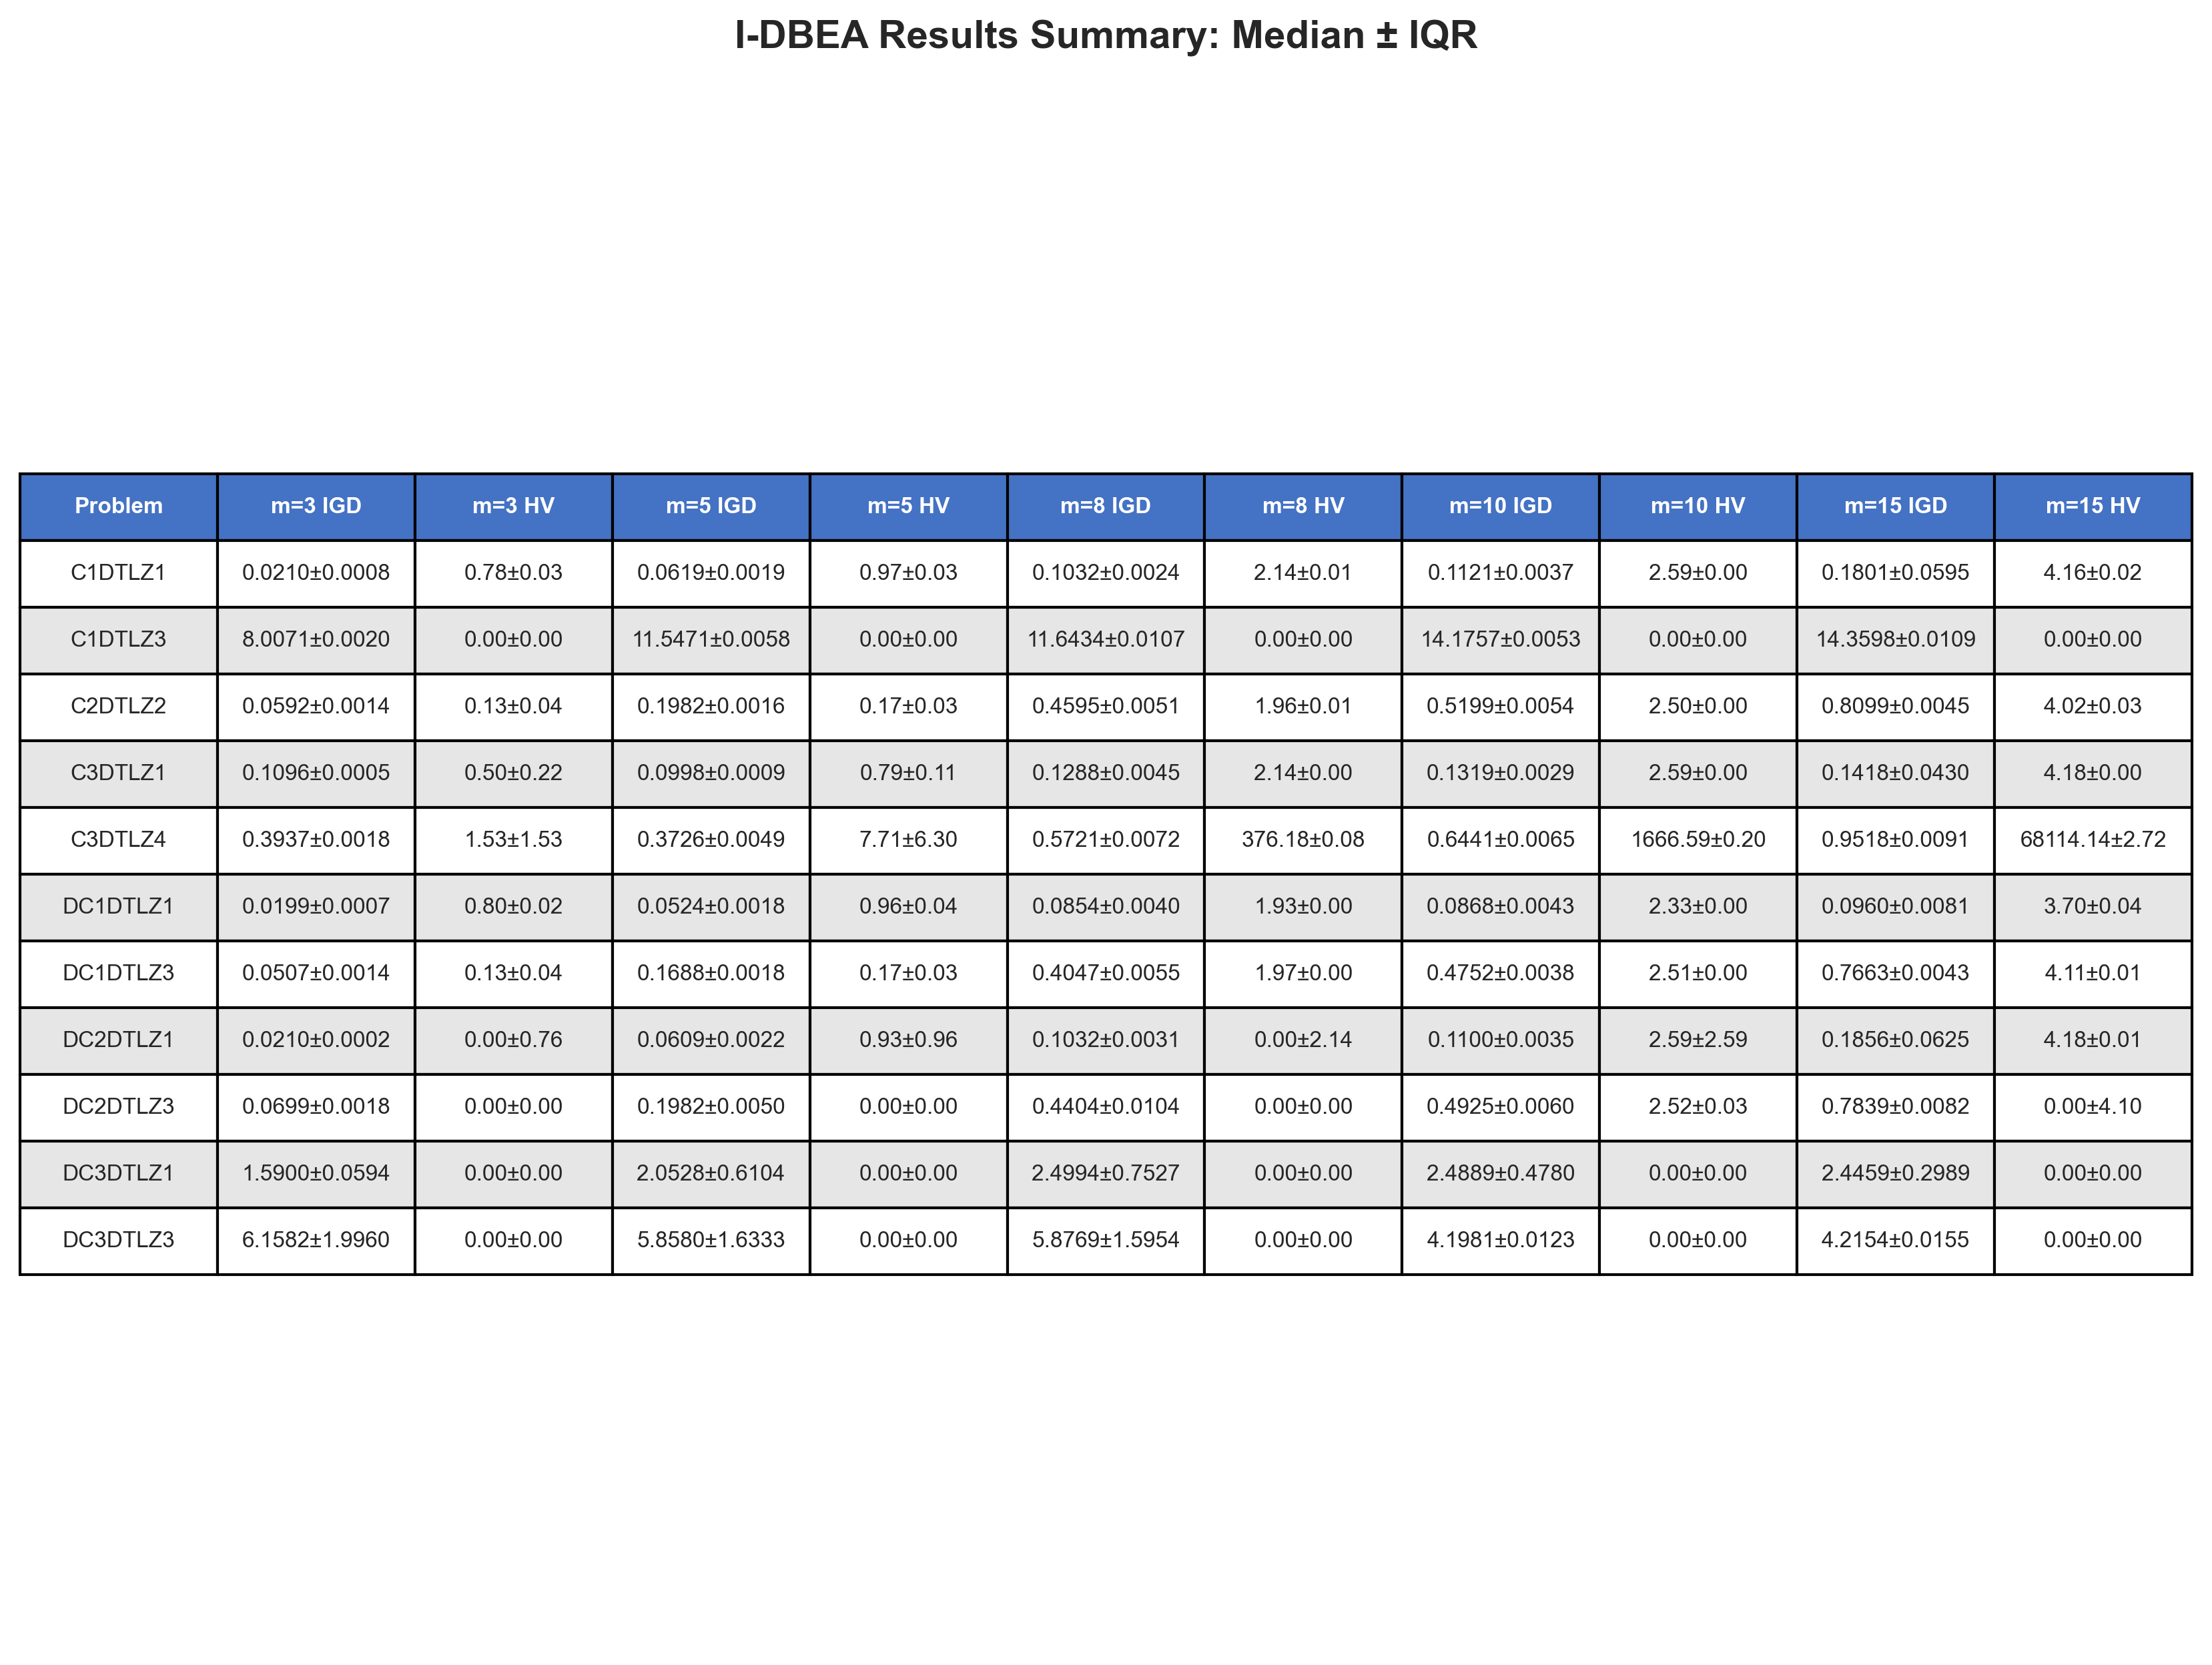
\includegraphics[width=0.85\textwidth]{summary_table.png}
    \caption{Results Summary }
\end{figure}


\end{document}